\subsection*{Supplementary figures for the house sparrow study}

We include figures containing the estimated relative importance of all covariates, and $R^2$ estimates, from the house sparrow study described in \Cref{sec:heritability_method} here. 

\begin{figure}[H]%\ContinuedFloat
  \centering
  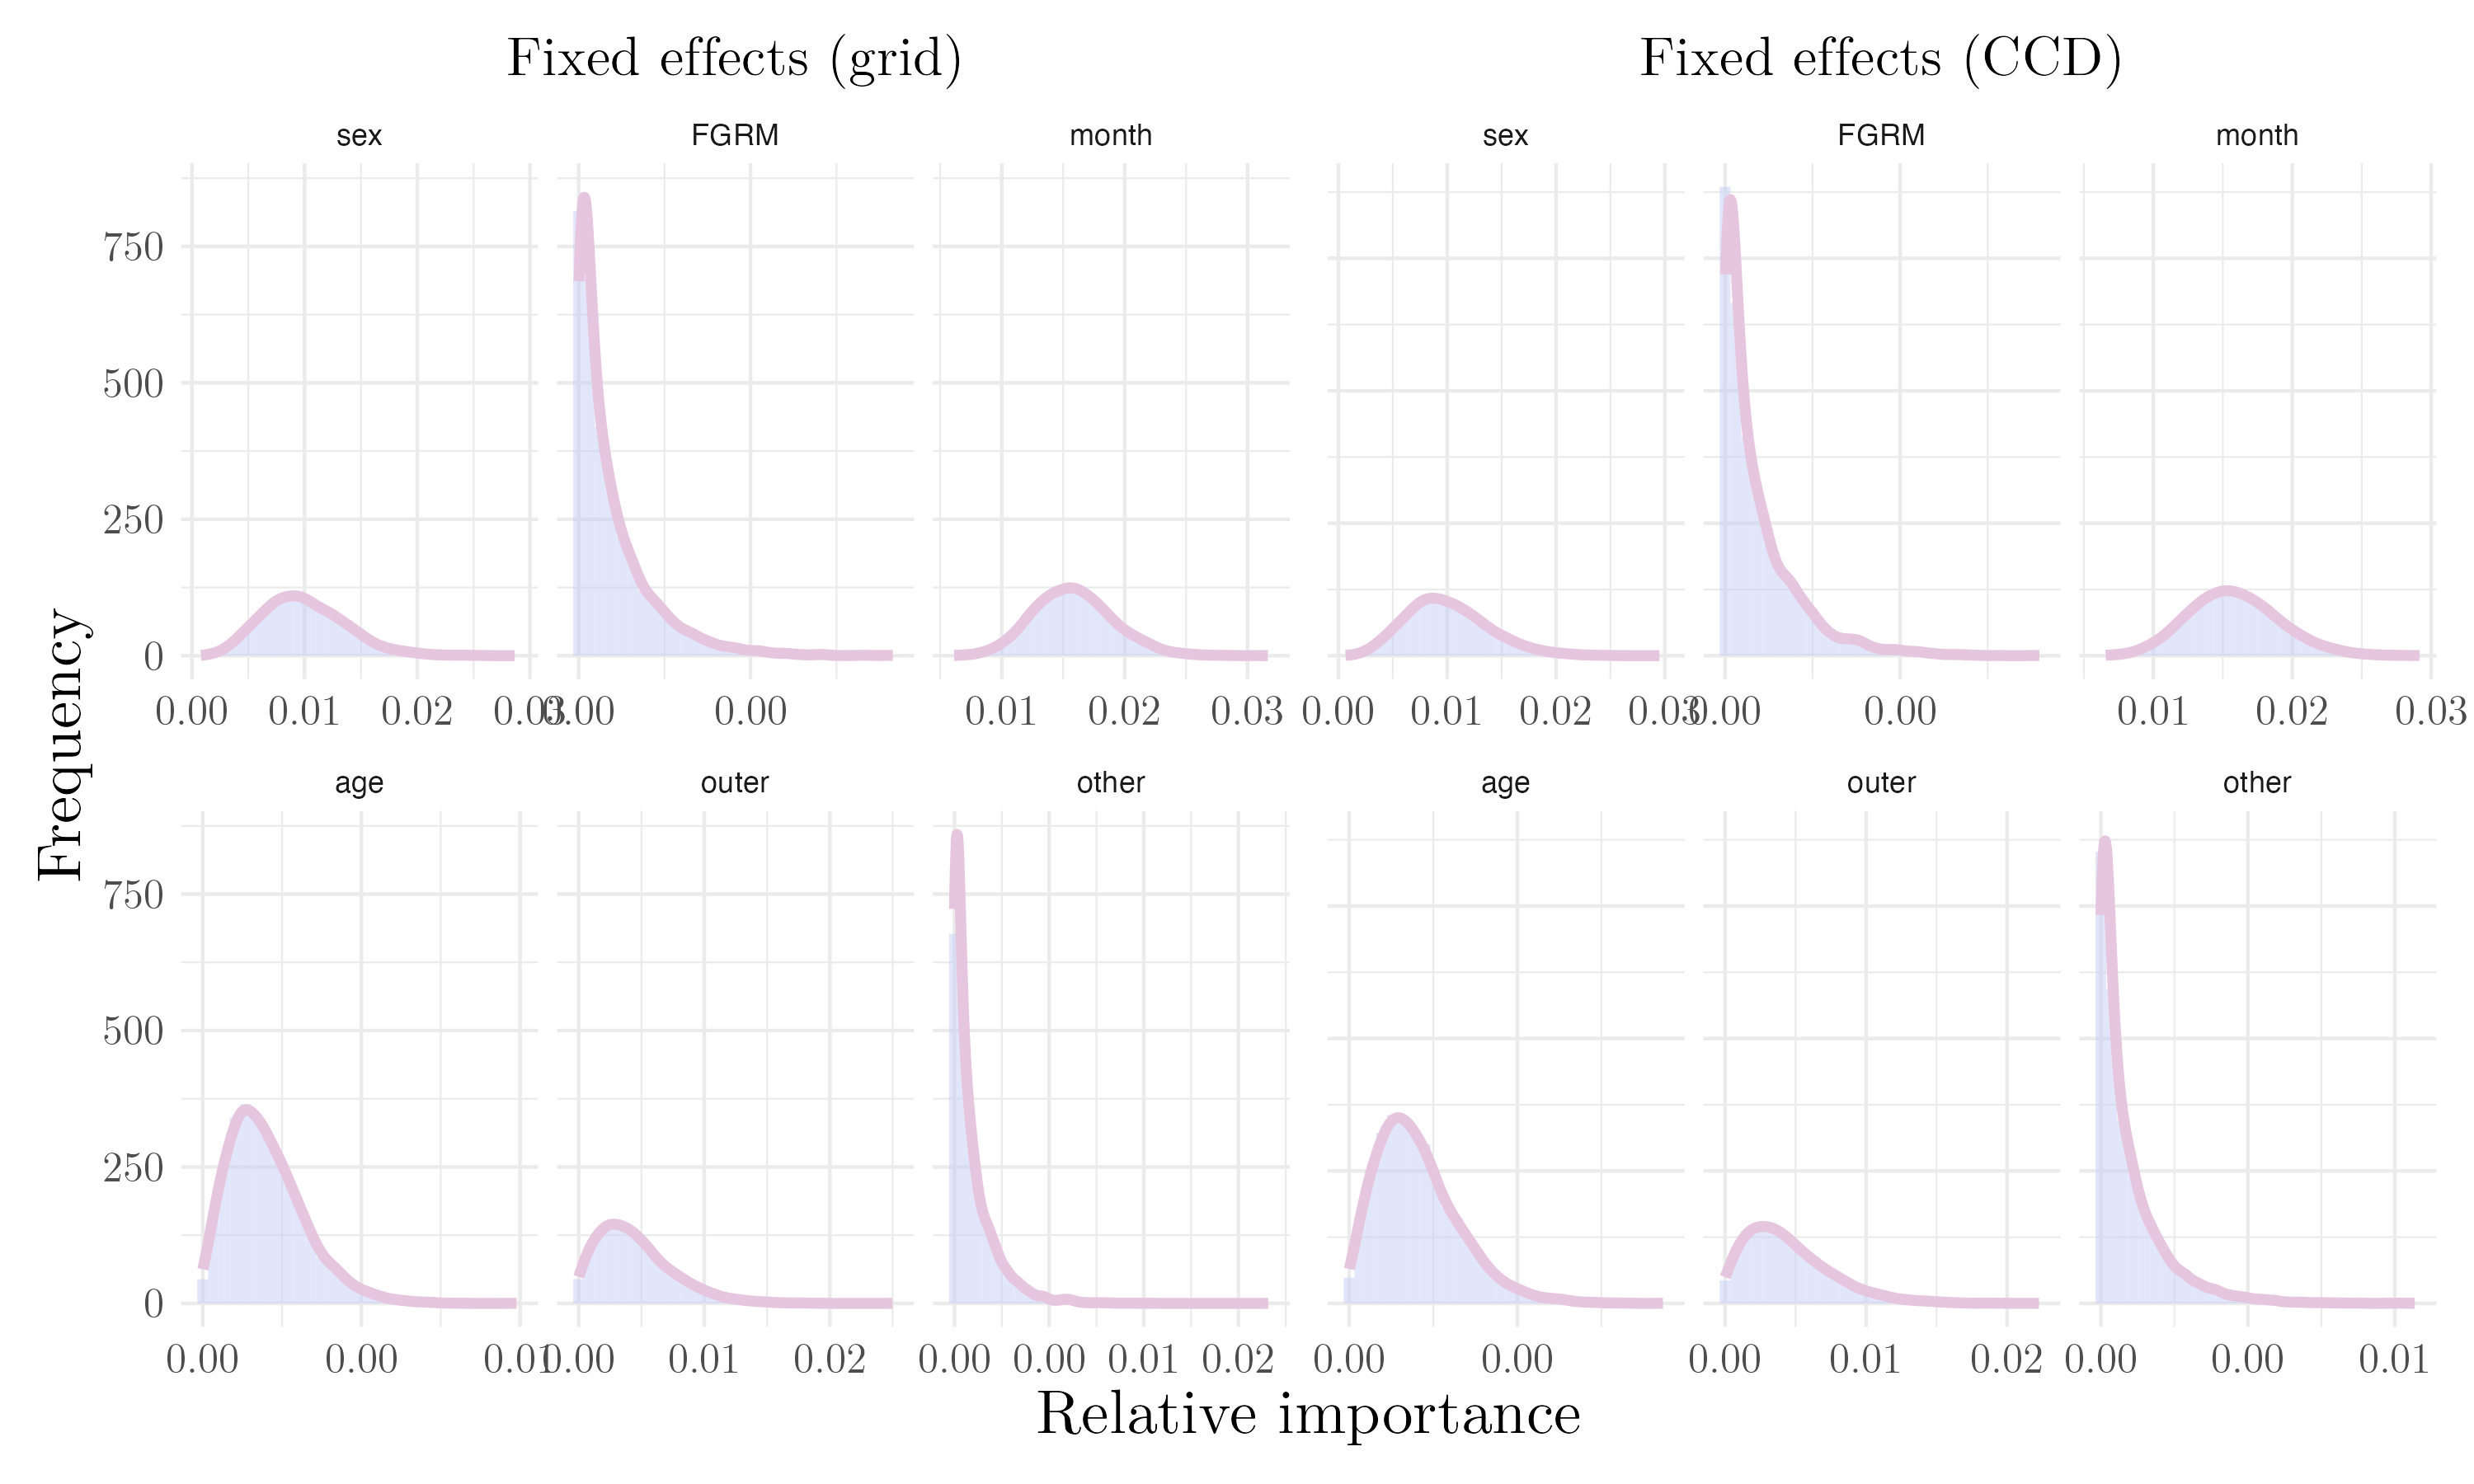
\includegraphics[width=1\linewidth]{Figures/House sparrow study/Mass_fixed.png}
  \caption[Posterior relative importance distributions of fixed effects in body mass model for house sparrow study]{Posterior relative importance distributions of fixed effects in body mass model for house sparrow study}
  \label{fig:mass_fixed_sparrows}
\end{figure}

\begin{figure}[H]%\ContinuedFloat
  \centering
  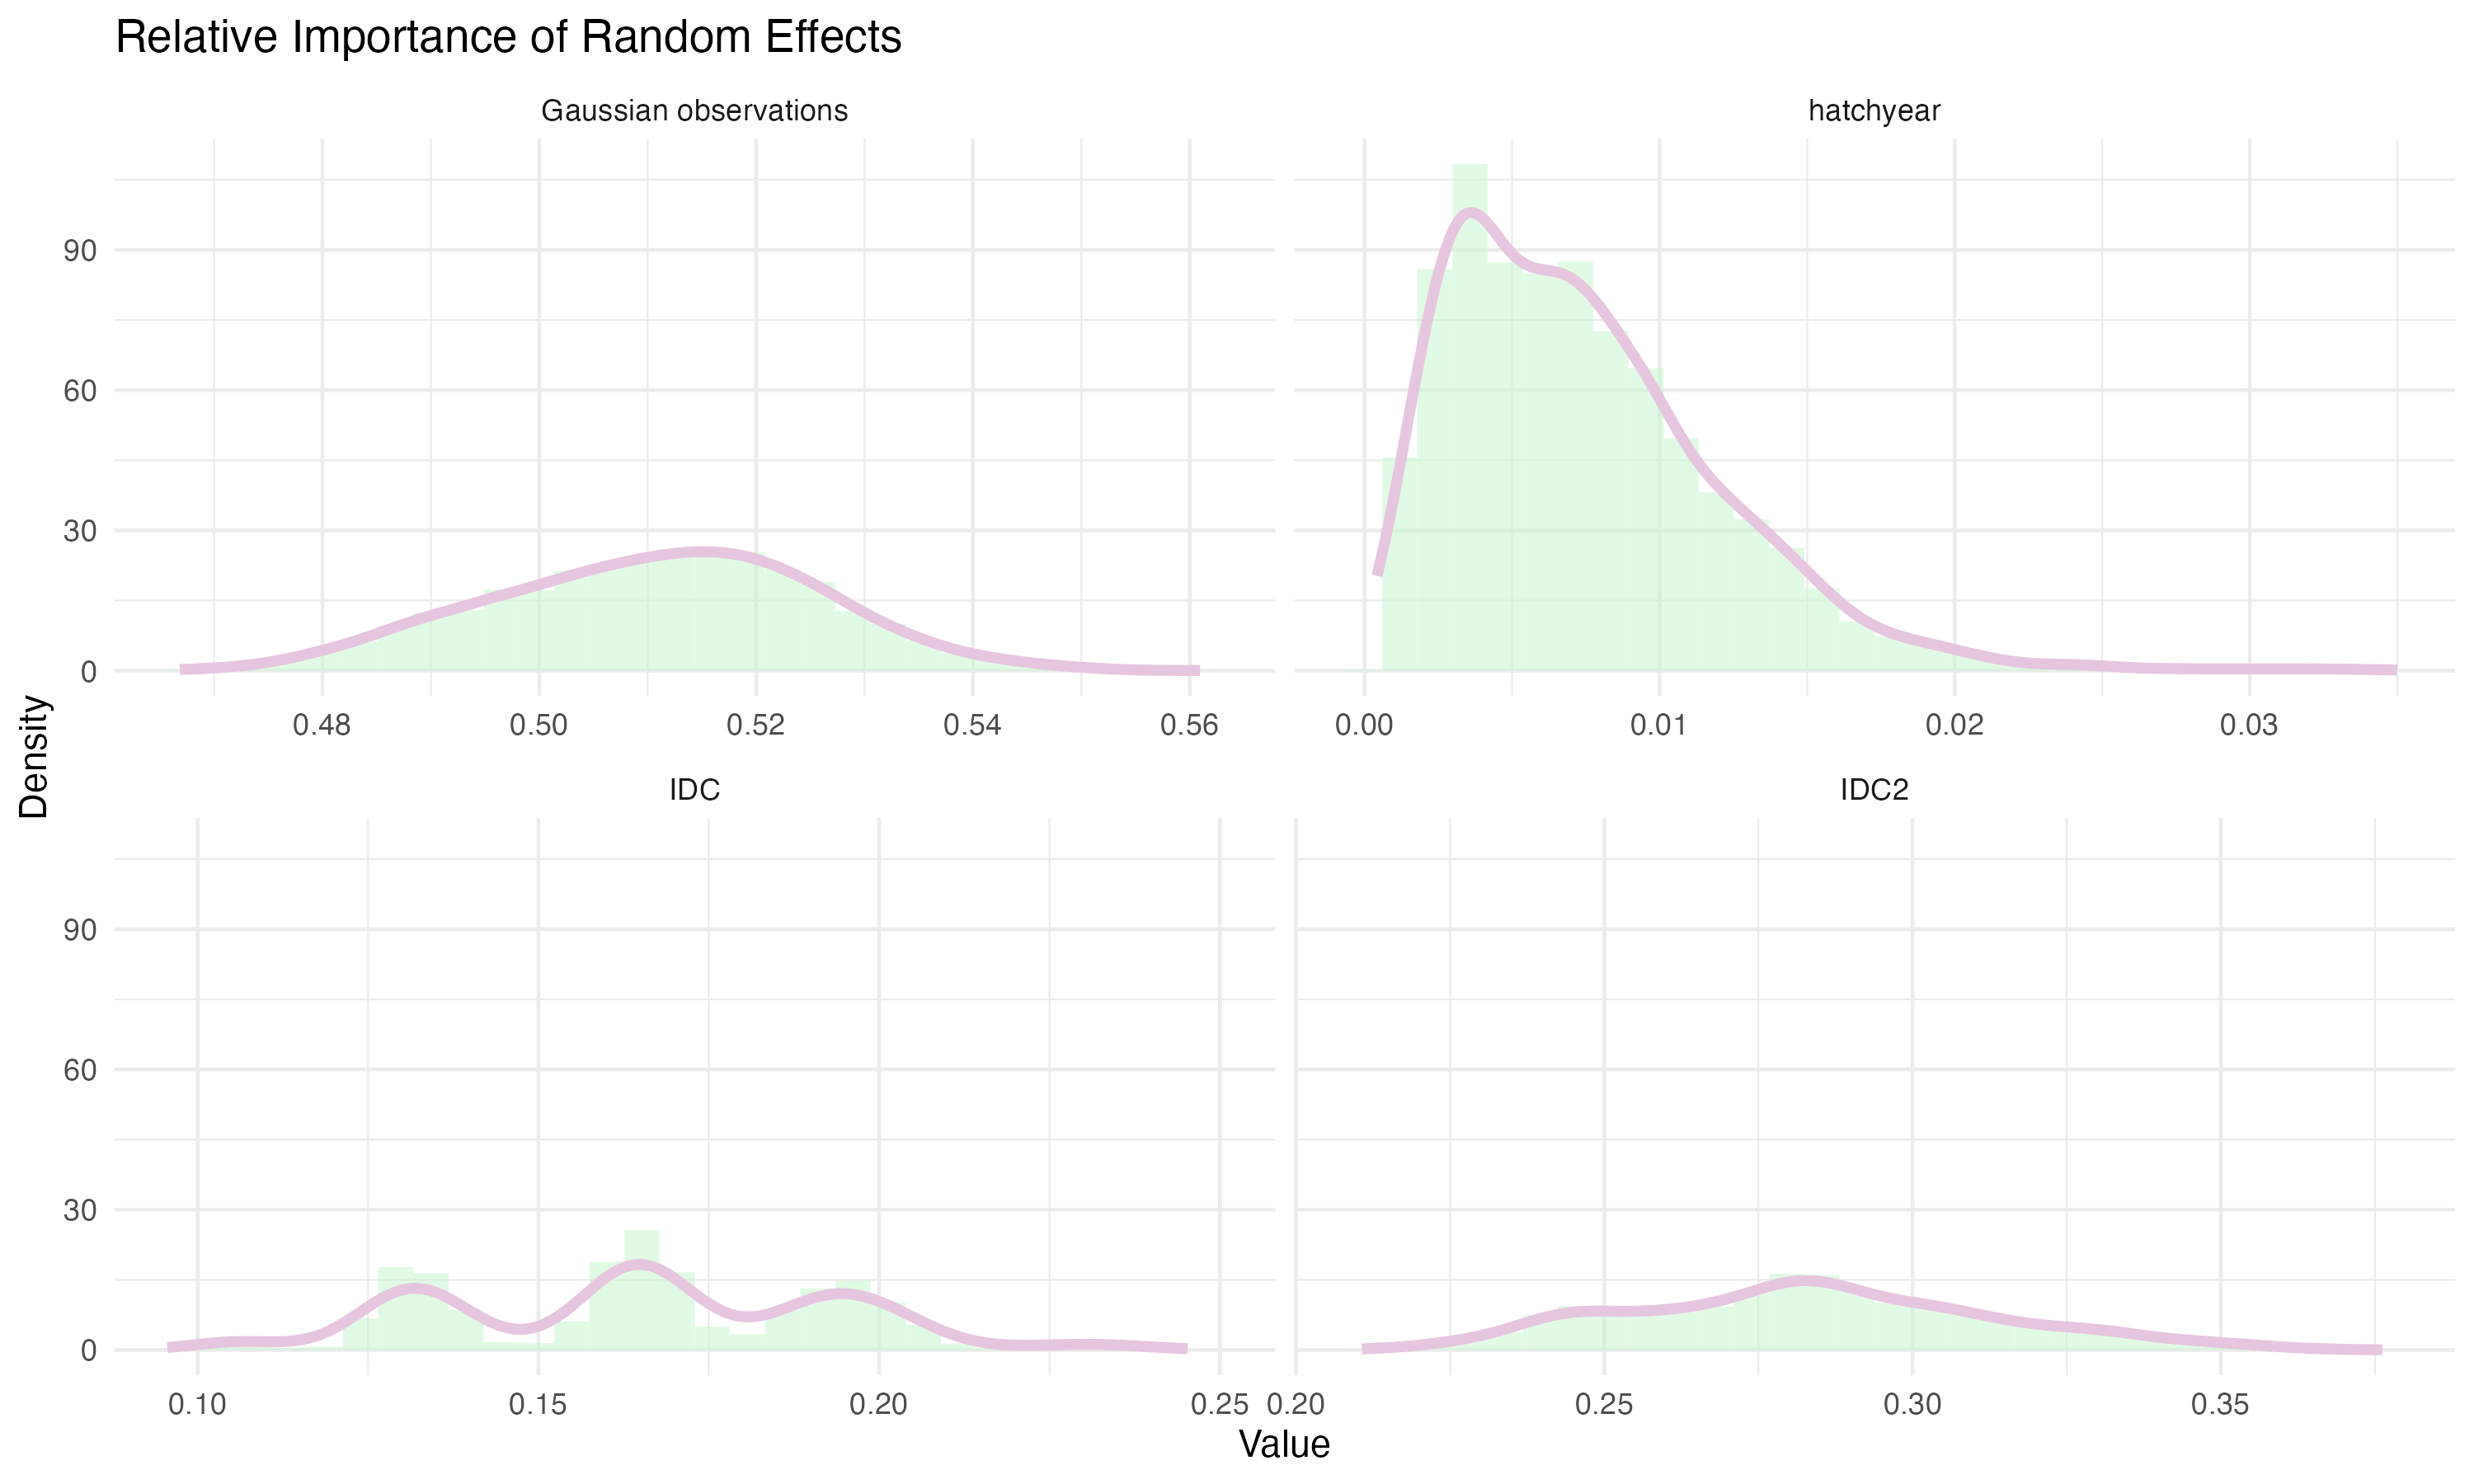
\includegraphics[width=1\linewidth]{Figures/House sparrow study/Mass_random.png}
  \caption[Posterior relative importance distributions of random effects in body mass model for house sparrow study]{Posterior relative importance distributions of random effects in body mass model for house sparrow study}
  \label{fig:mass_random_sparrows}
\end{figure}

\begin{figure}[H]%\ContinuedFloat
  \centering
  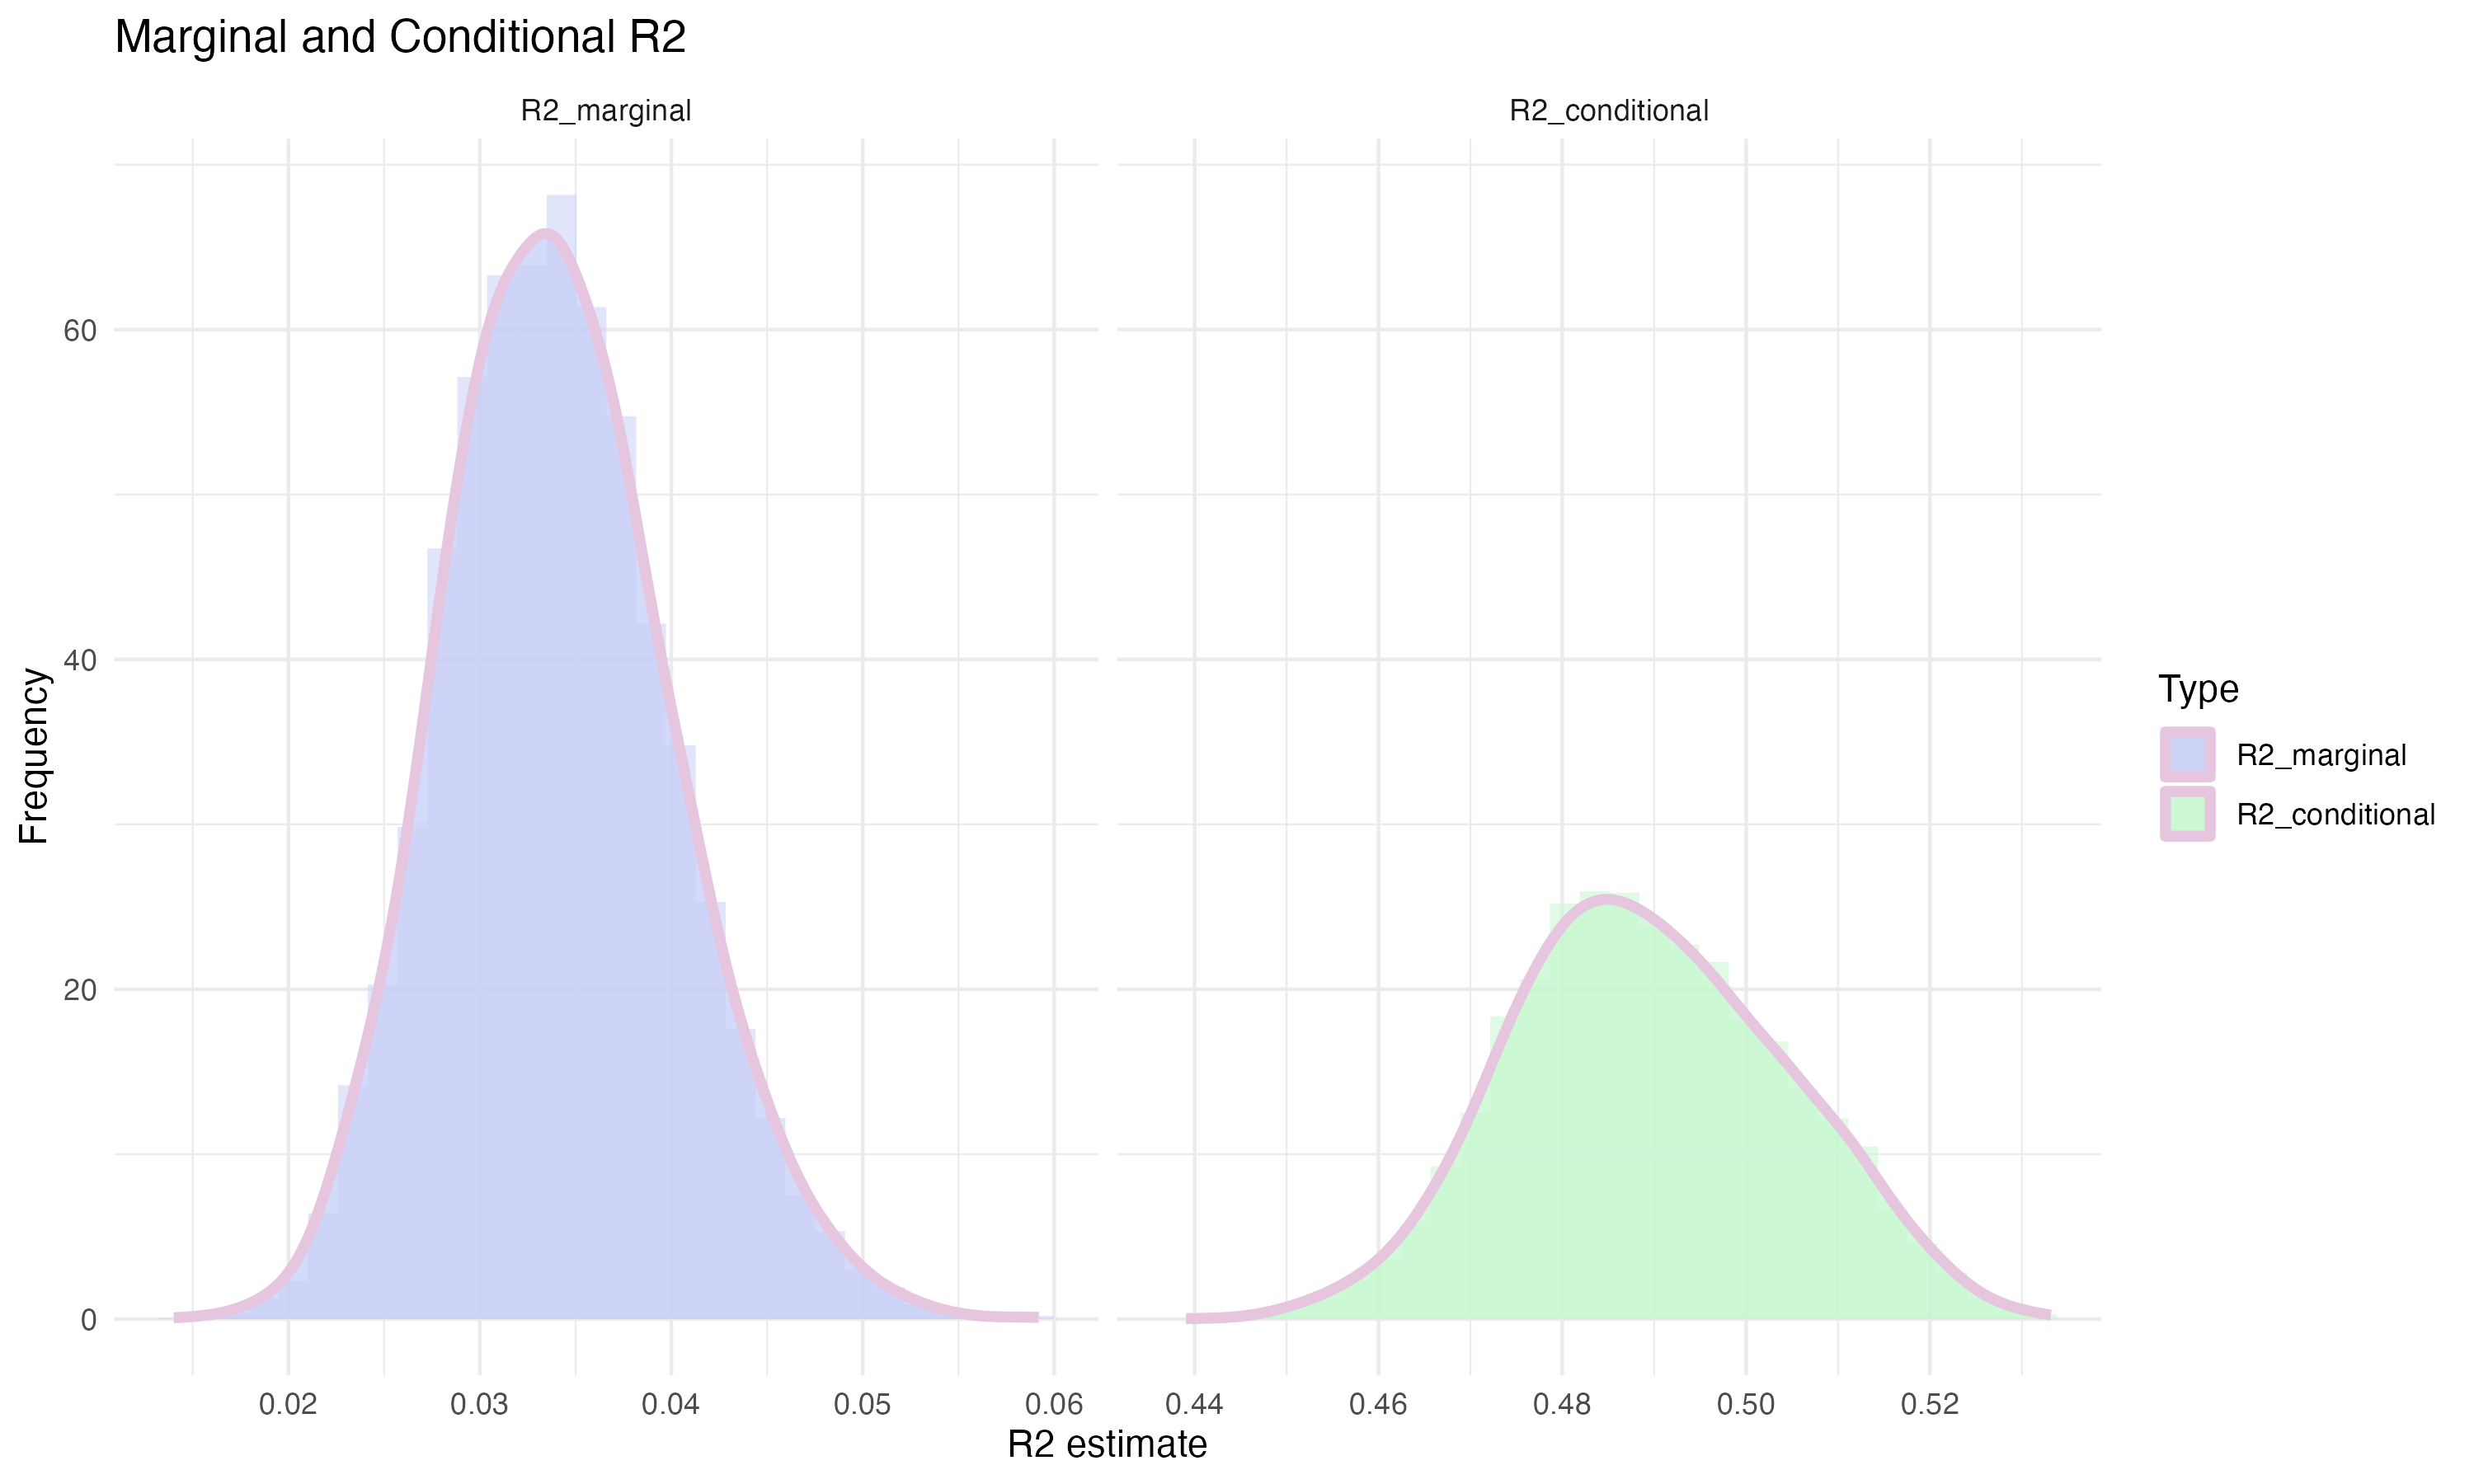
\includegraphics[width=1\linewidth]{Figures/House sparrow study/Mass_r2.png}
  \caption[Posterior distributions of $R^2$ values in body mass model for house sparrow study]{Posterior distributions of $R^2$ values in body mass model for house sparrow study}
  \label{fig:mass_r2}
\end{figure}

\begin{figure}[H]%\ContinuedFloat
  \centering
  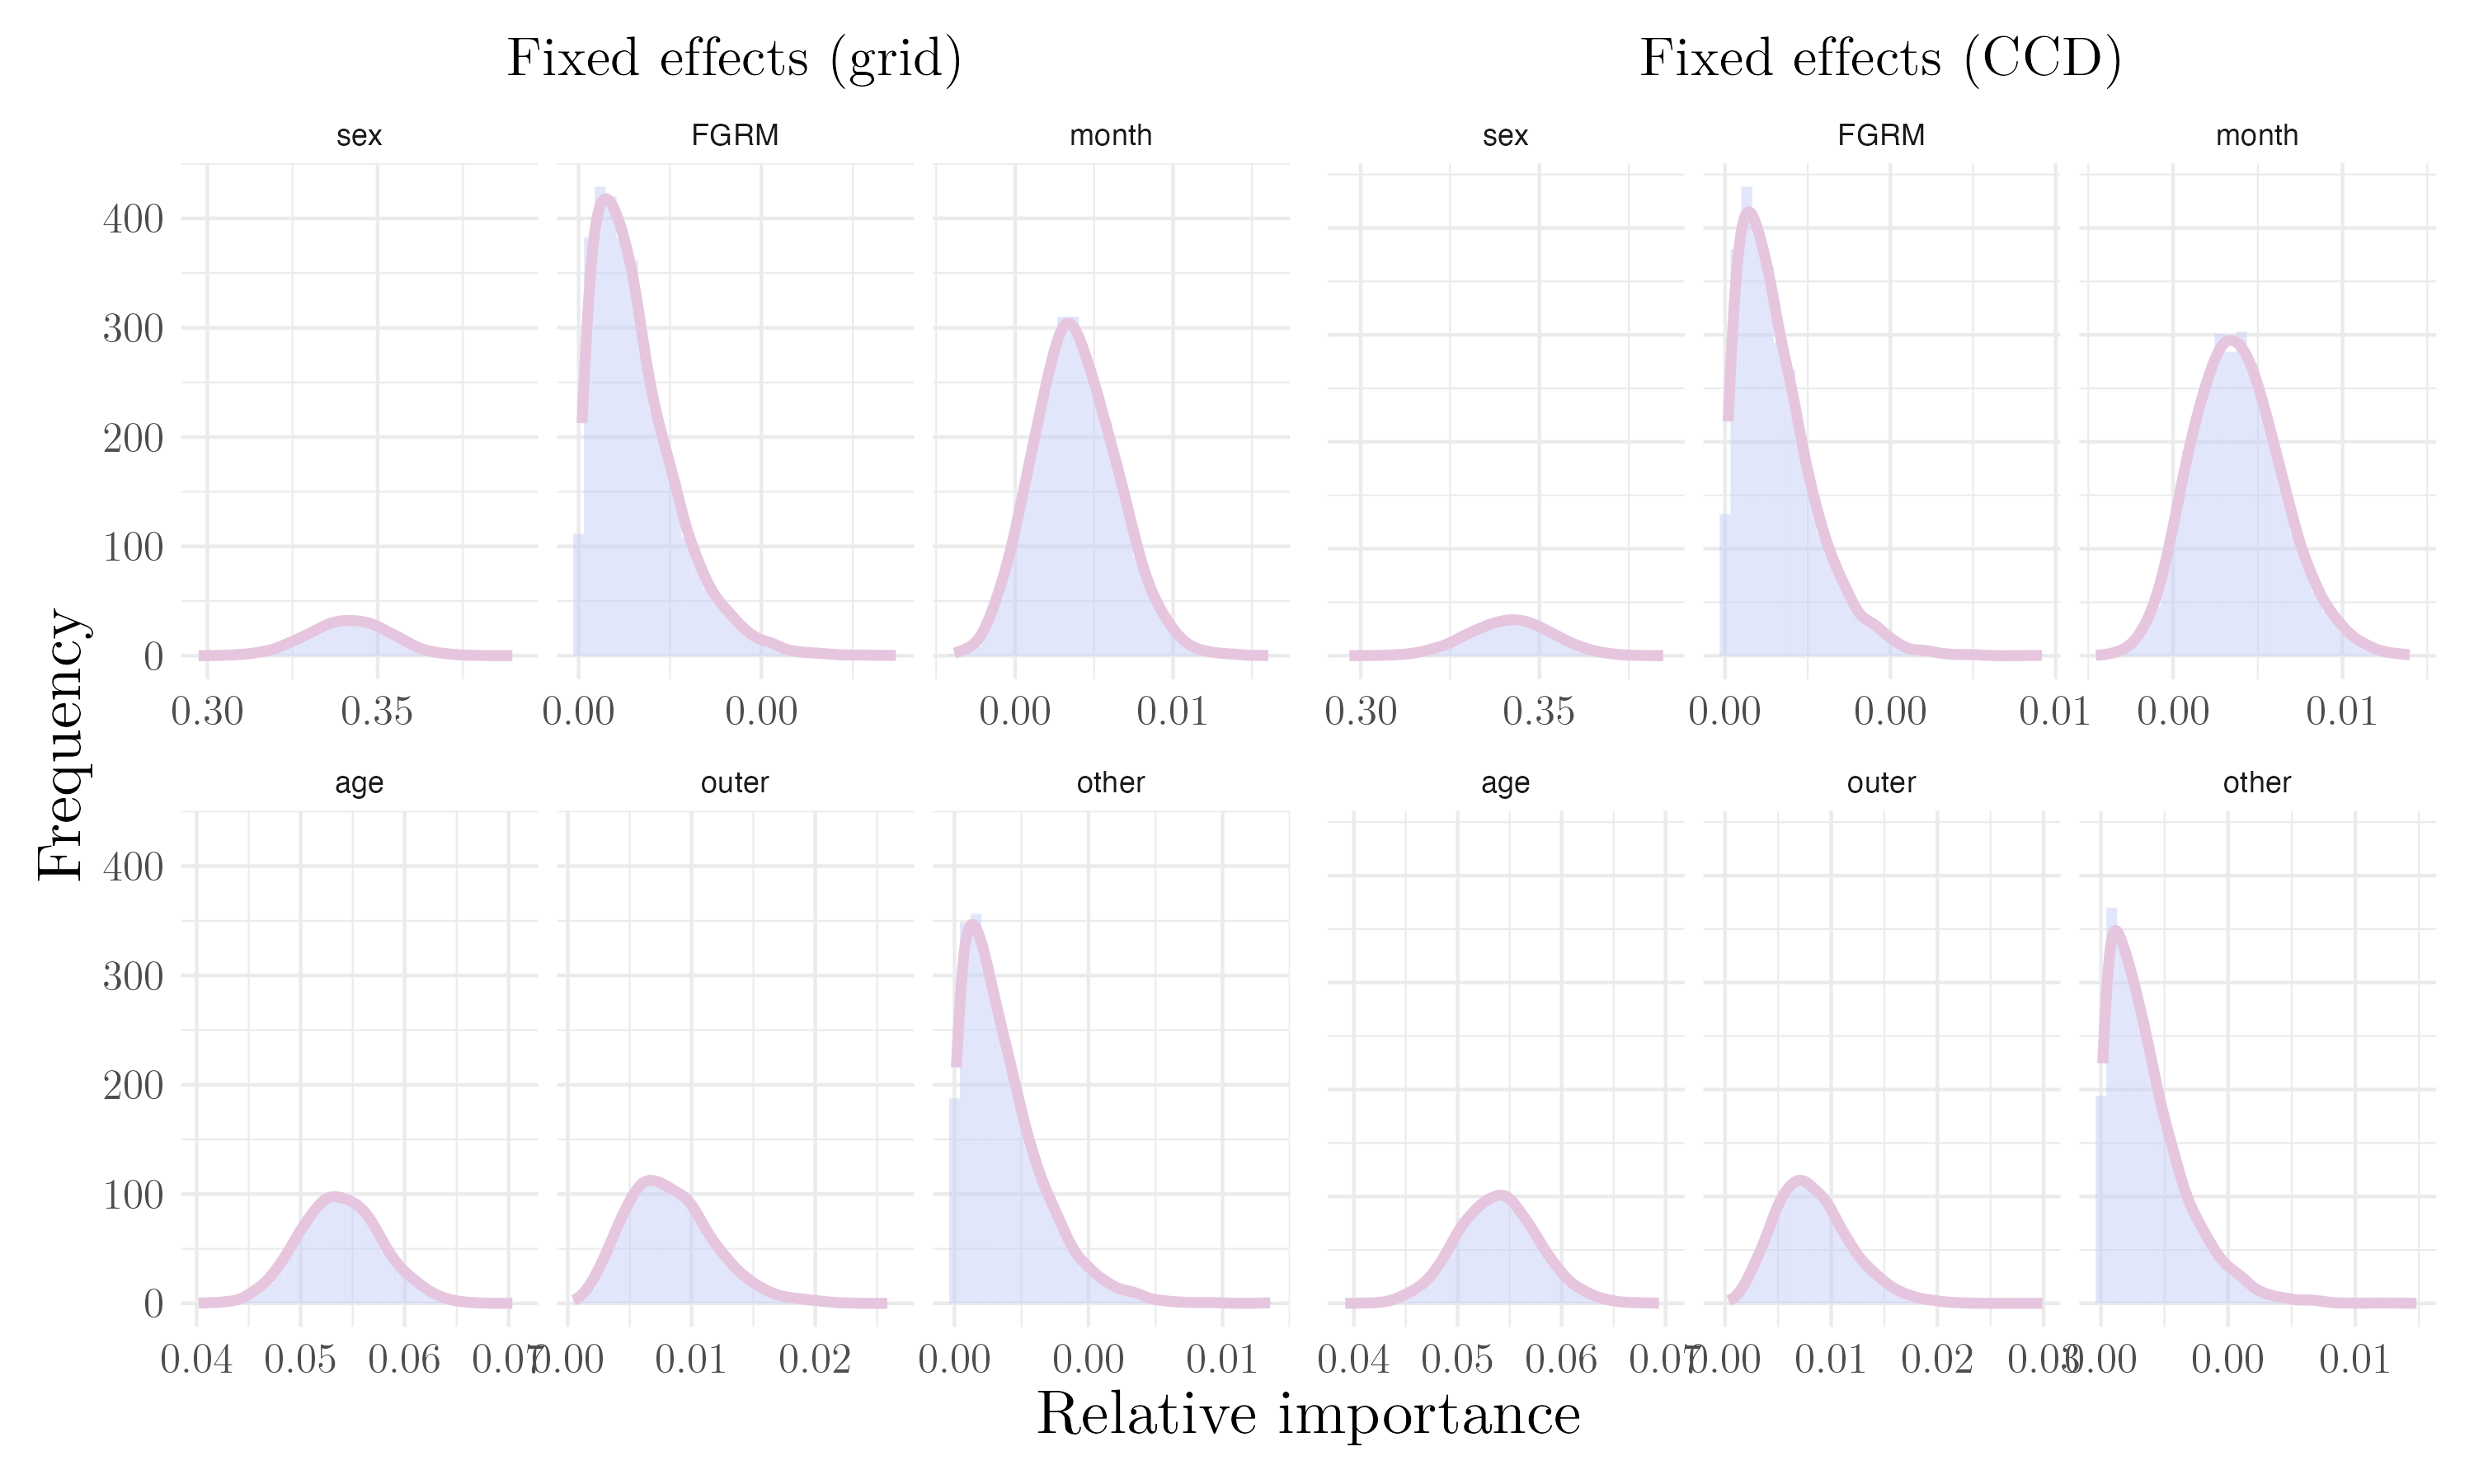
\includegraphics[width=1\linewidth]{Figures/House sparrow study/Wing_fixed.png}
  \caption[Posterior relative importance distributions of fixed effects in wing length model for house sparrow study]{Posterior relative importance distributions of fixed effects in wing length model for house sparrow study}
  \label{fig:wing_fixed_sparrows}
\end{figure}

\begin{figure}[H]%\ContinuedFloat
  \centering
  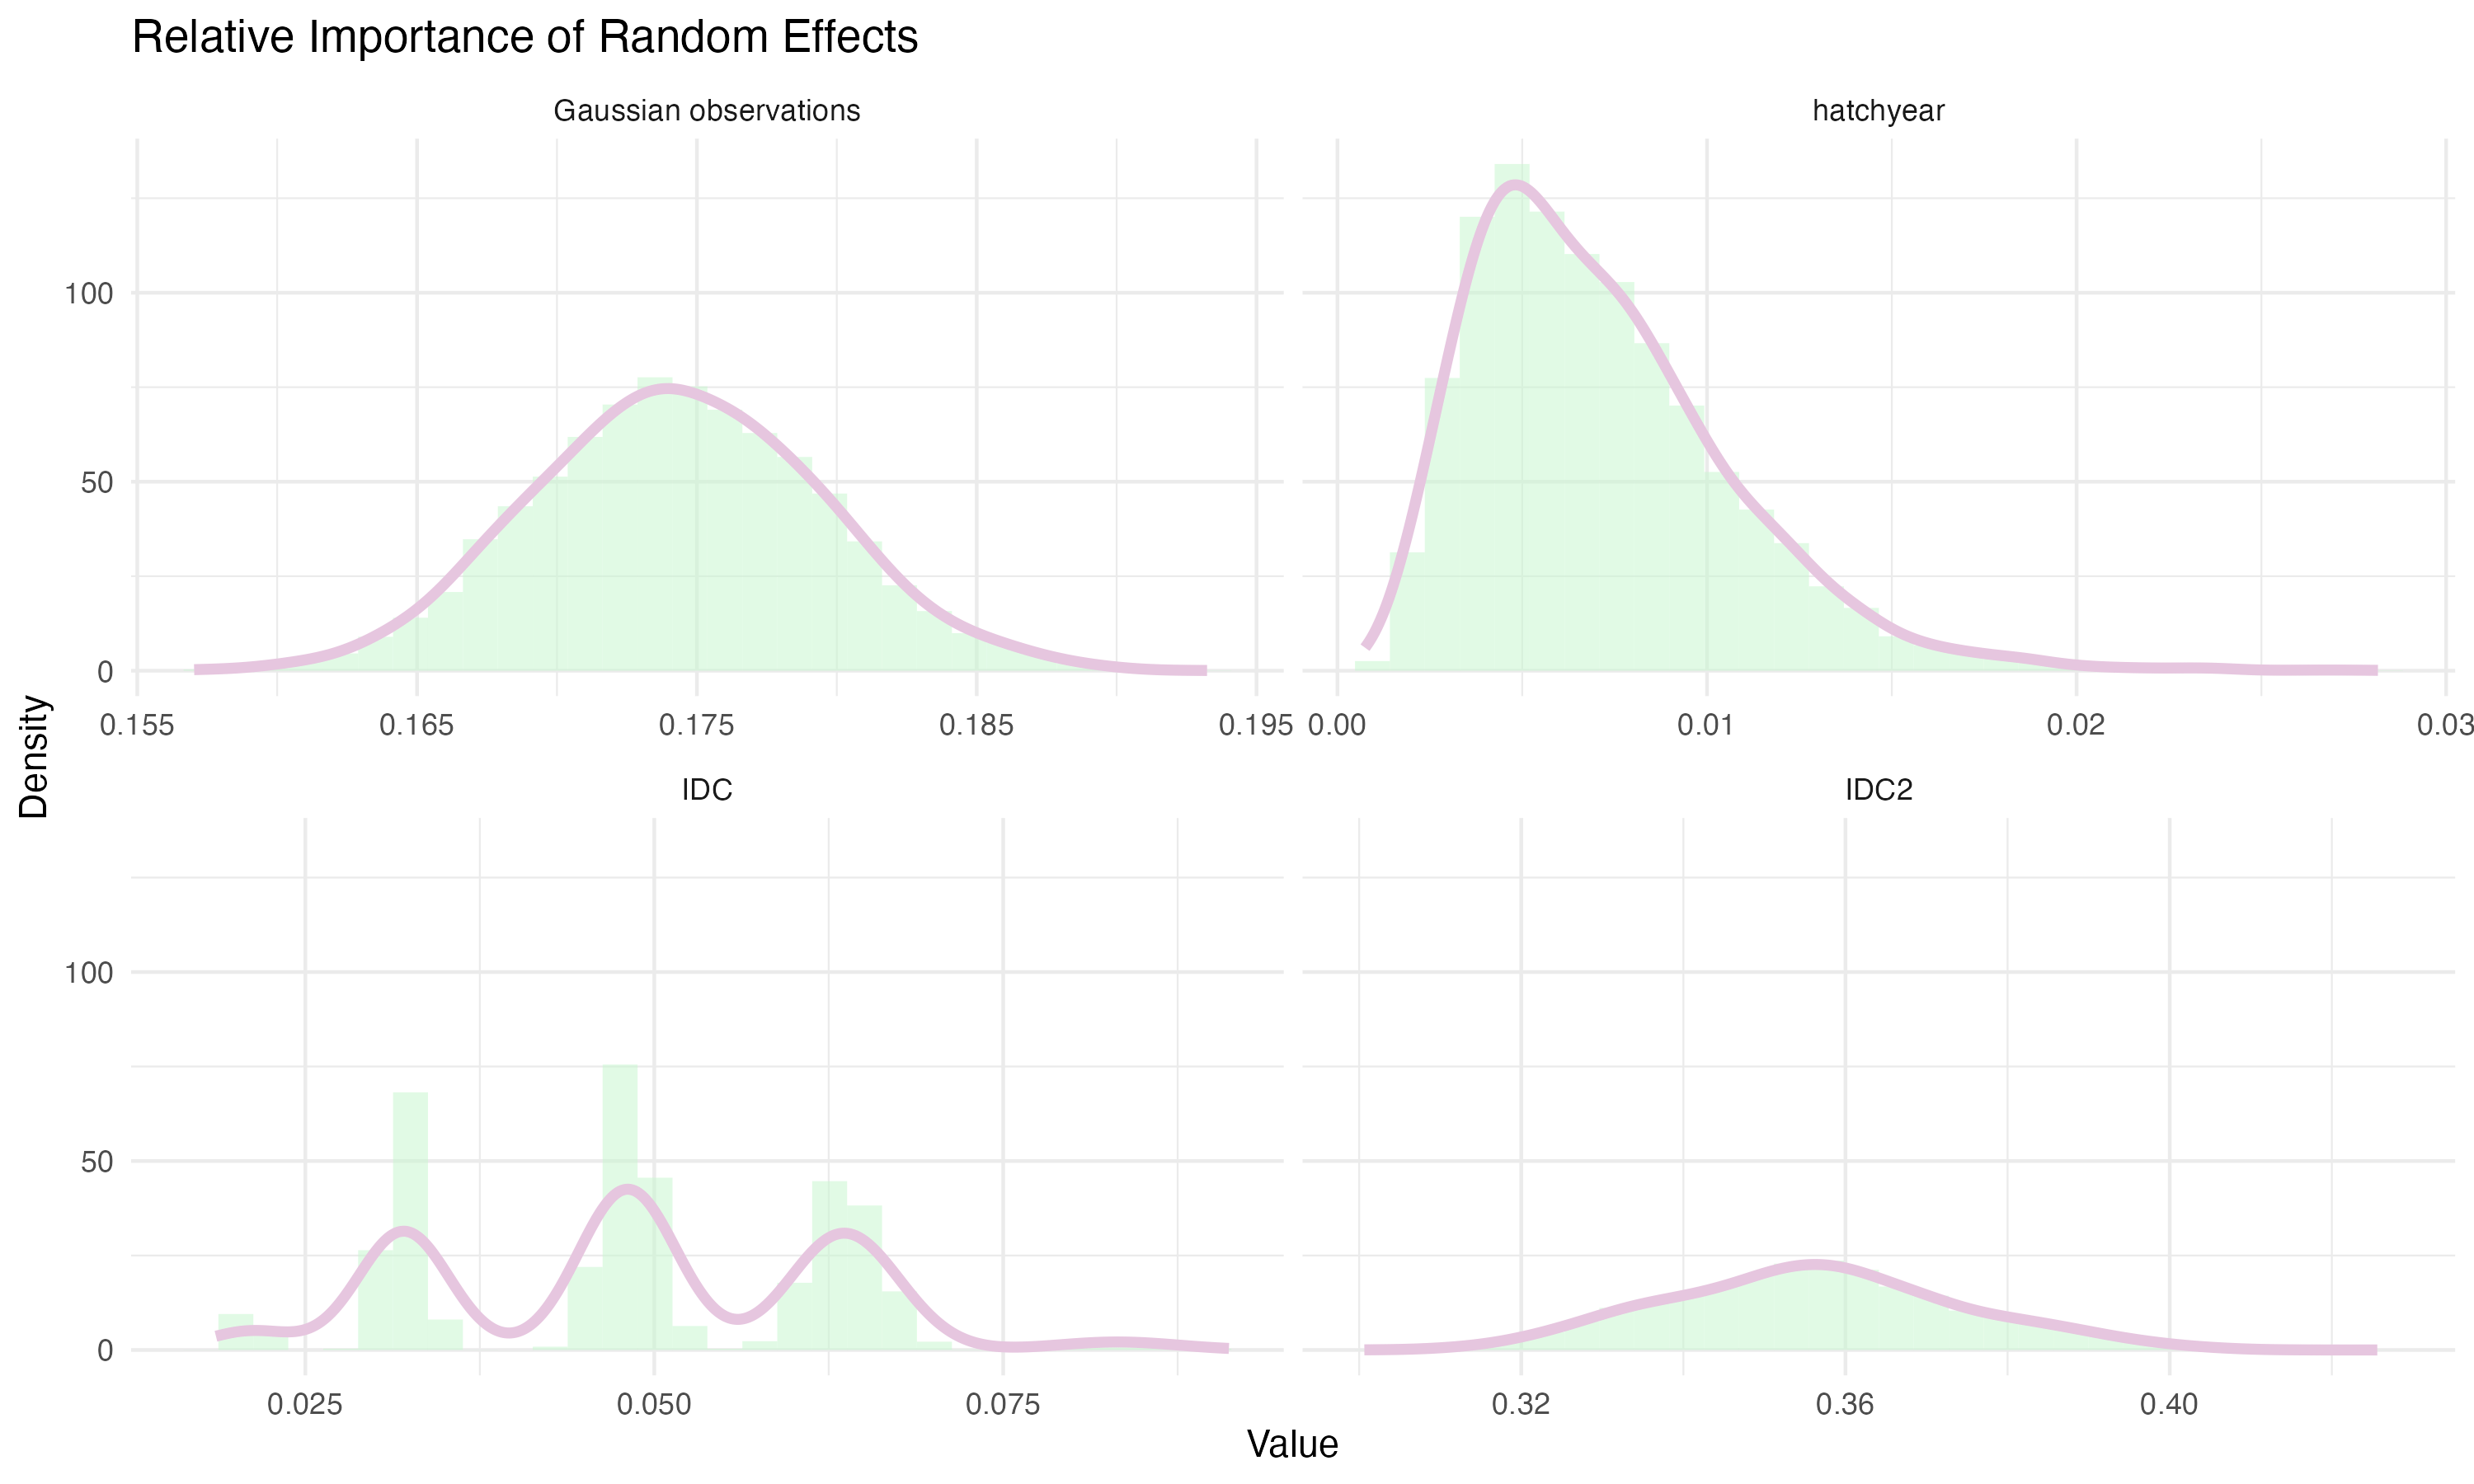
\includegraphics[width=1\linewidth]{Figures/House sparrow study/Wing_random.png}
  \caption[Posterior relative importance distributions of random effects in wing length model for house sparrow study]{Posterior relative importance distributions of random effects in wing length model for house sparrow study}
  \label{fig:wing_random_sparrows}
\end{figure}

\begin{figure}[H]%\ContinuedFloat
  \centering
  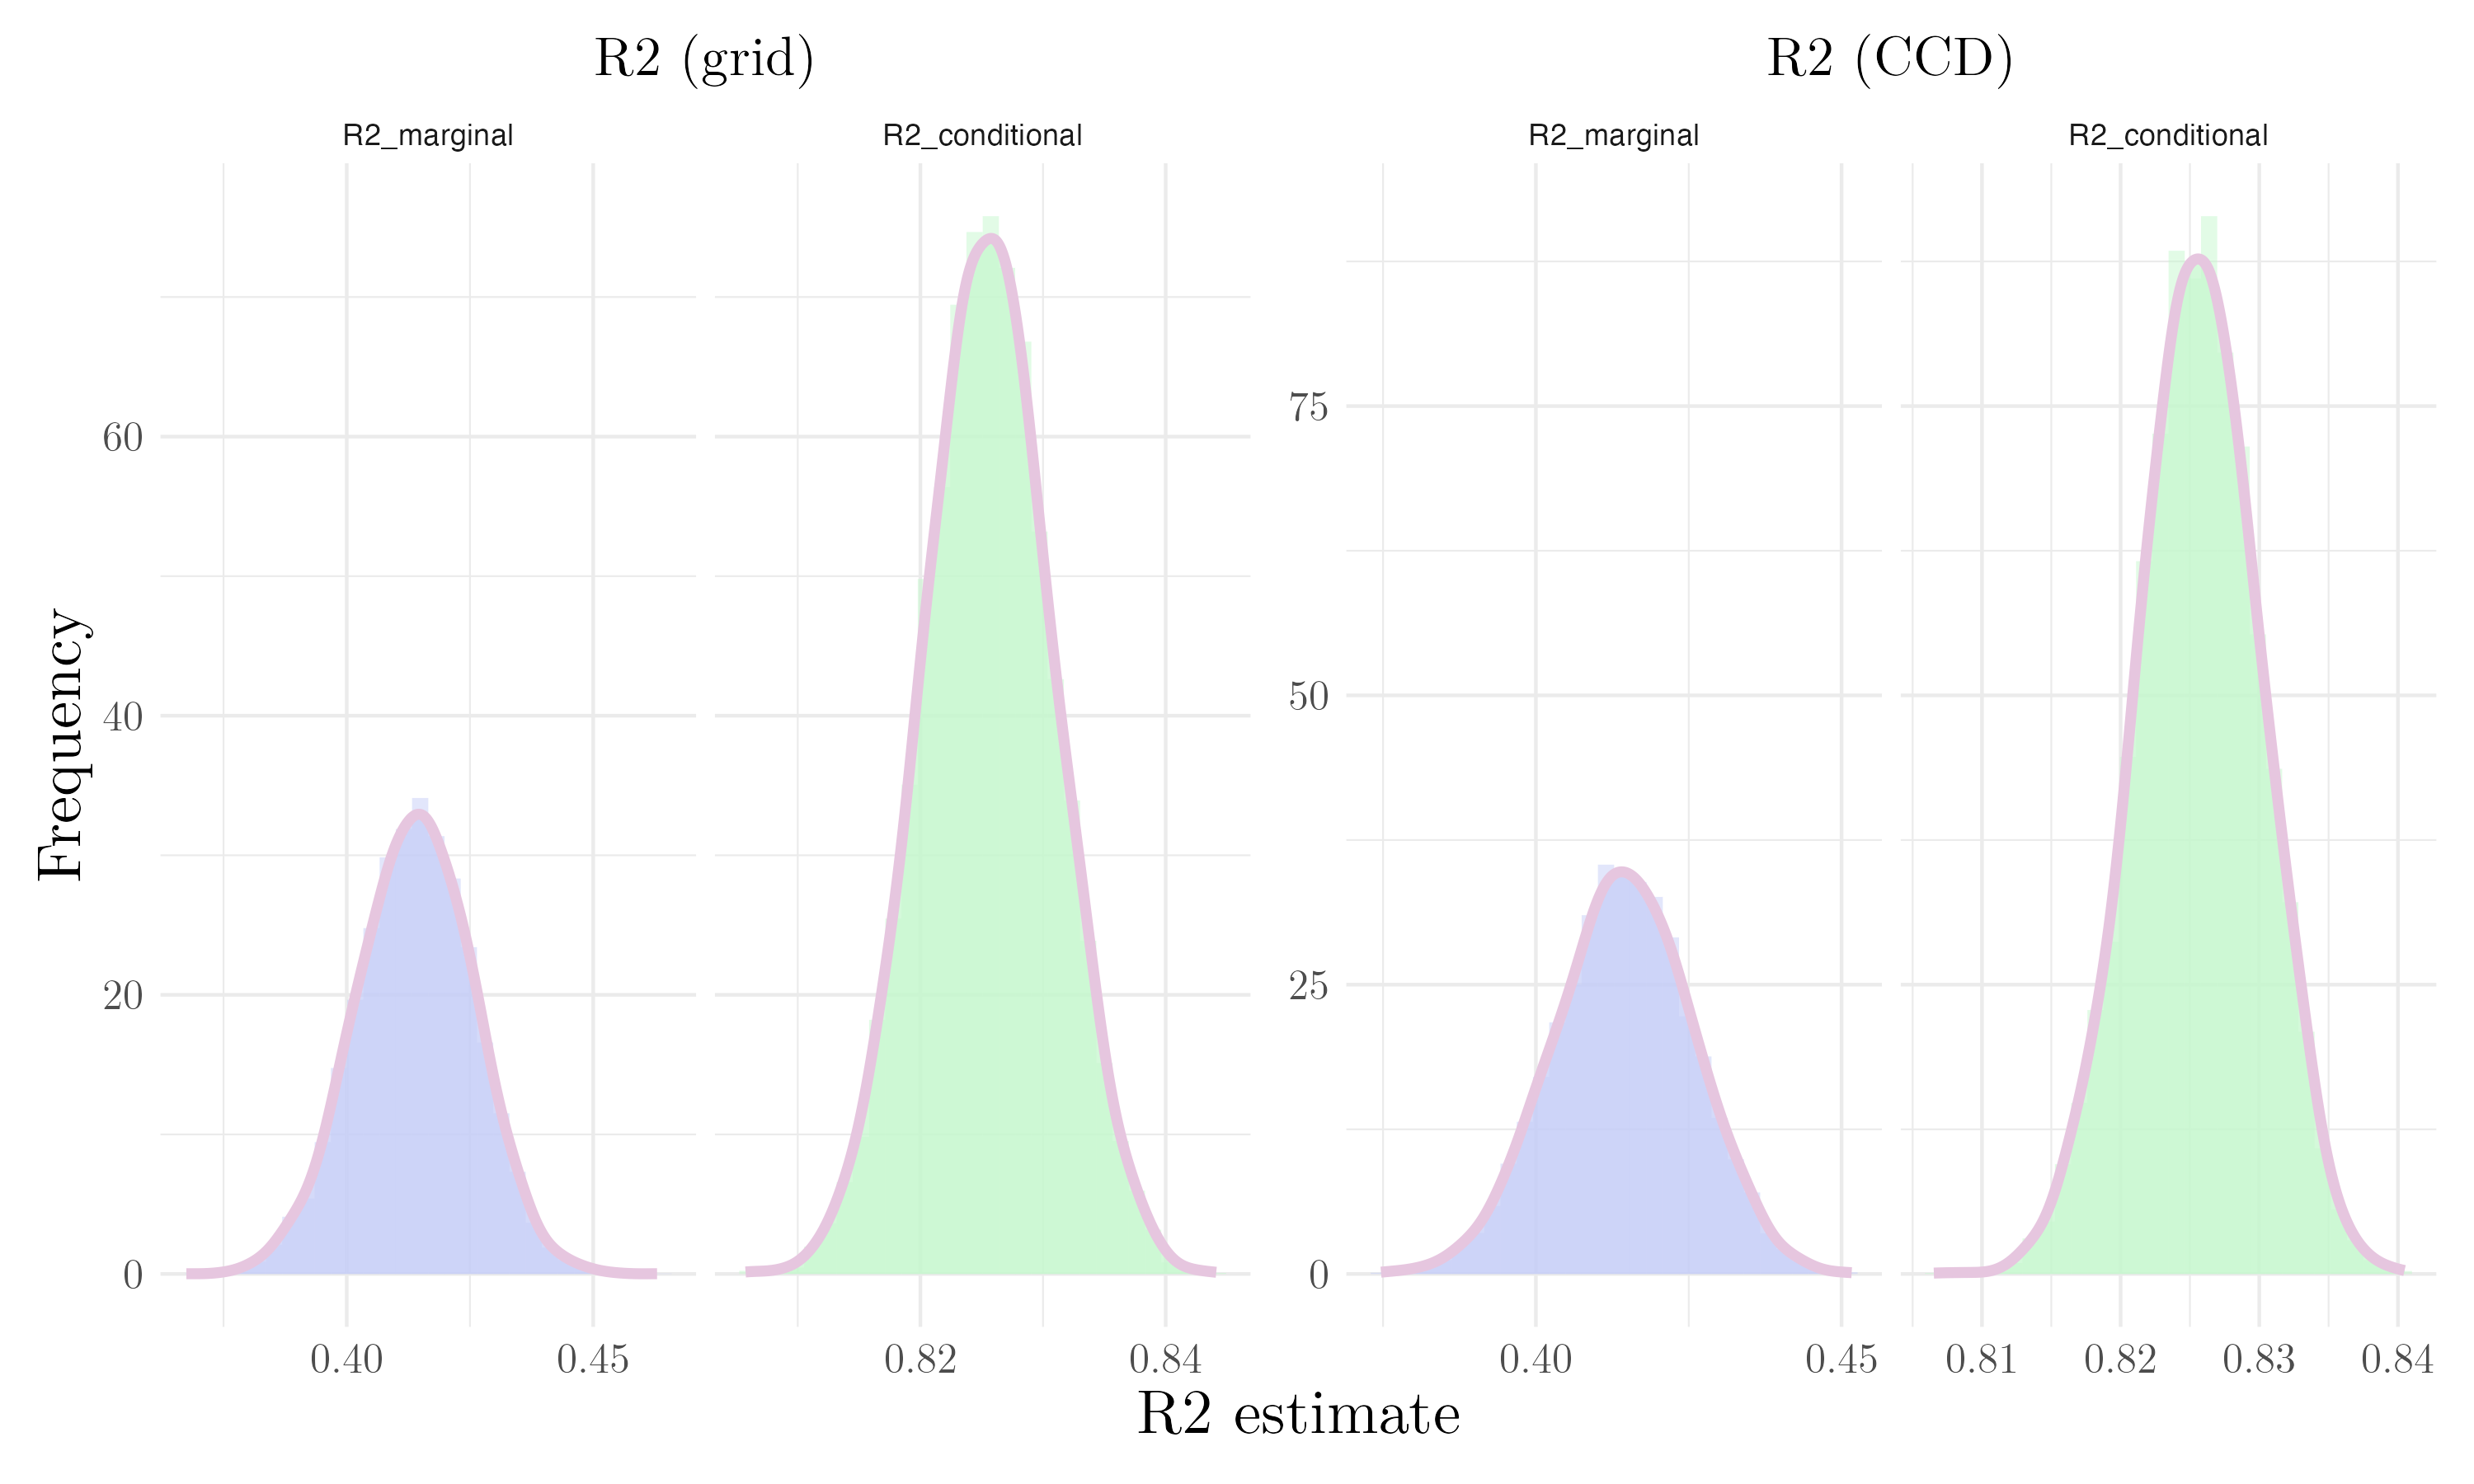
\includegraphics[width=1\linewidth]{Figures/House sparrow study/Wing_r2.png}
  \caption[Posterior distributions of $R^2$ values in wing length model for house sparrow study]{Posterior distributions of $R^2$ values in wing length model for house sparrow study}
  \label{fig:wing_r2}
\end{figure}

\begin{figure}[H]%\ContinuedFloat
  \centering
  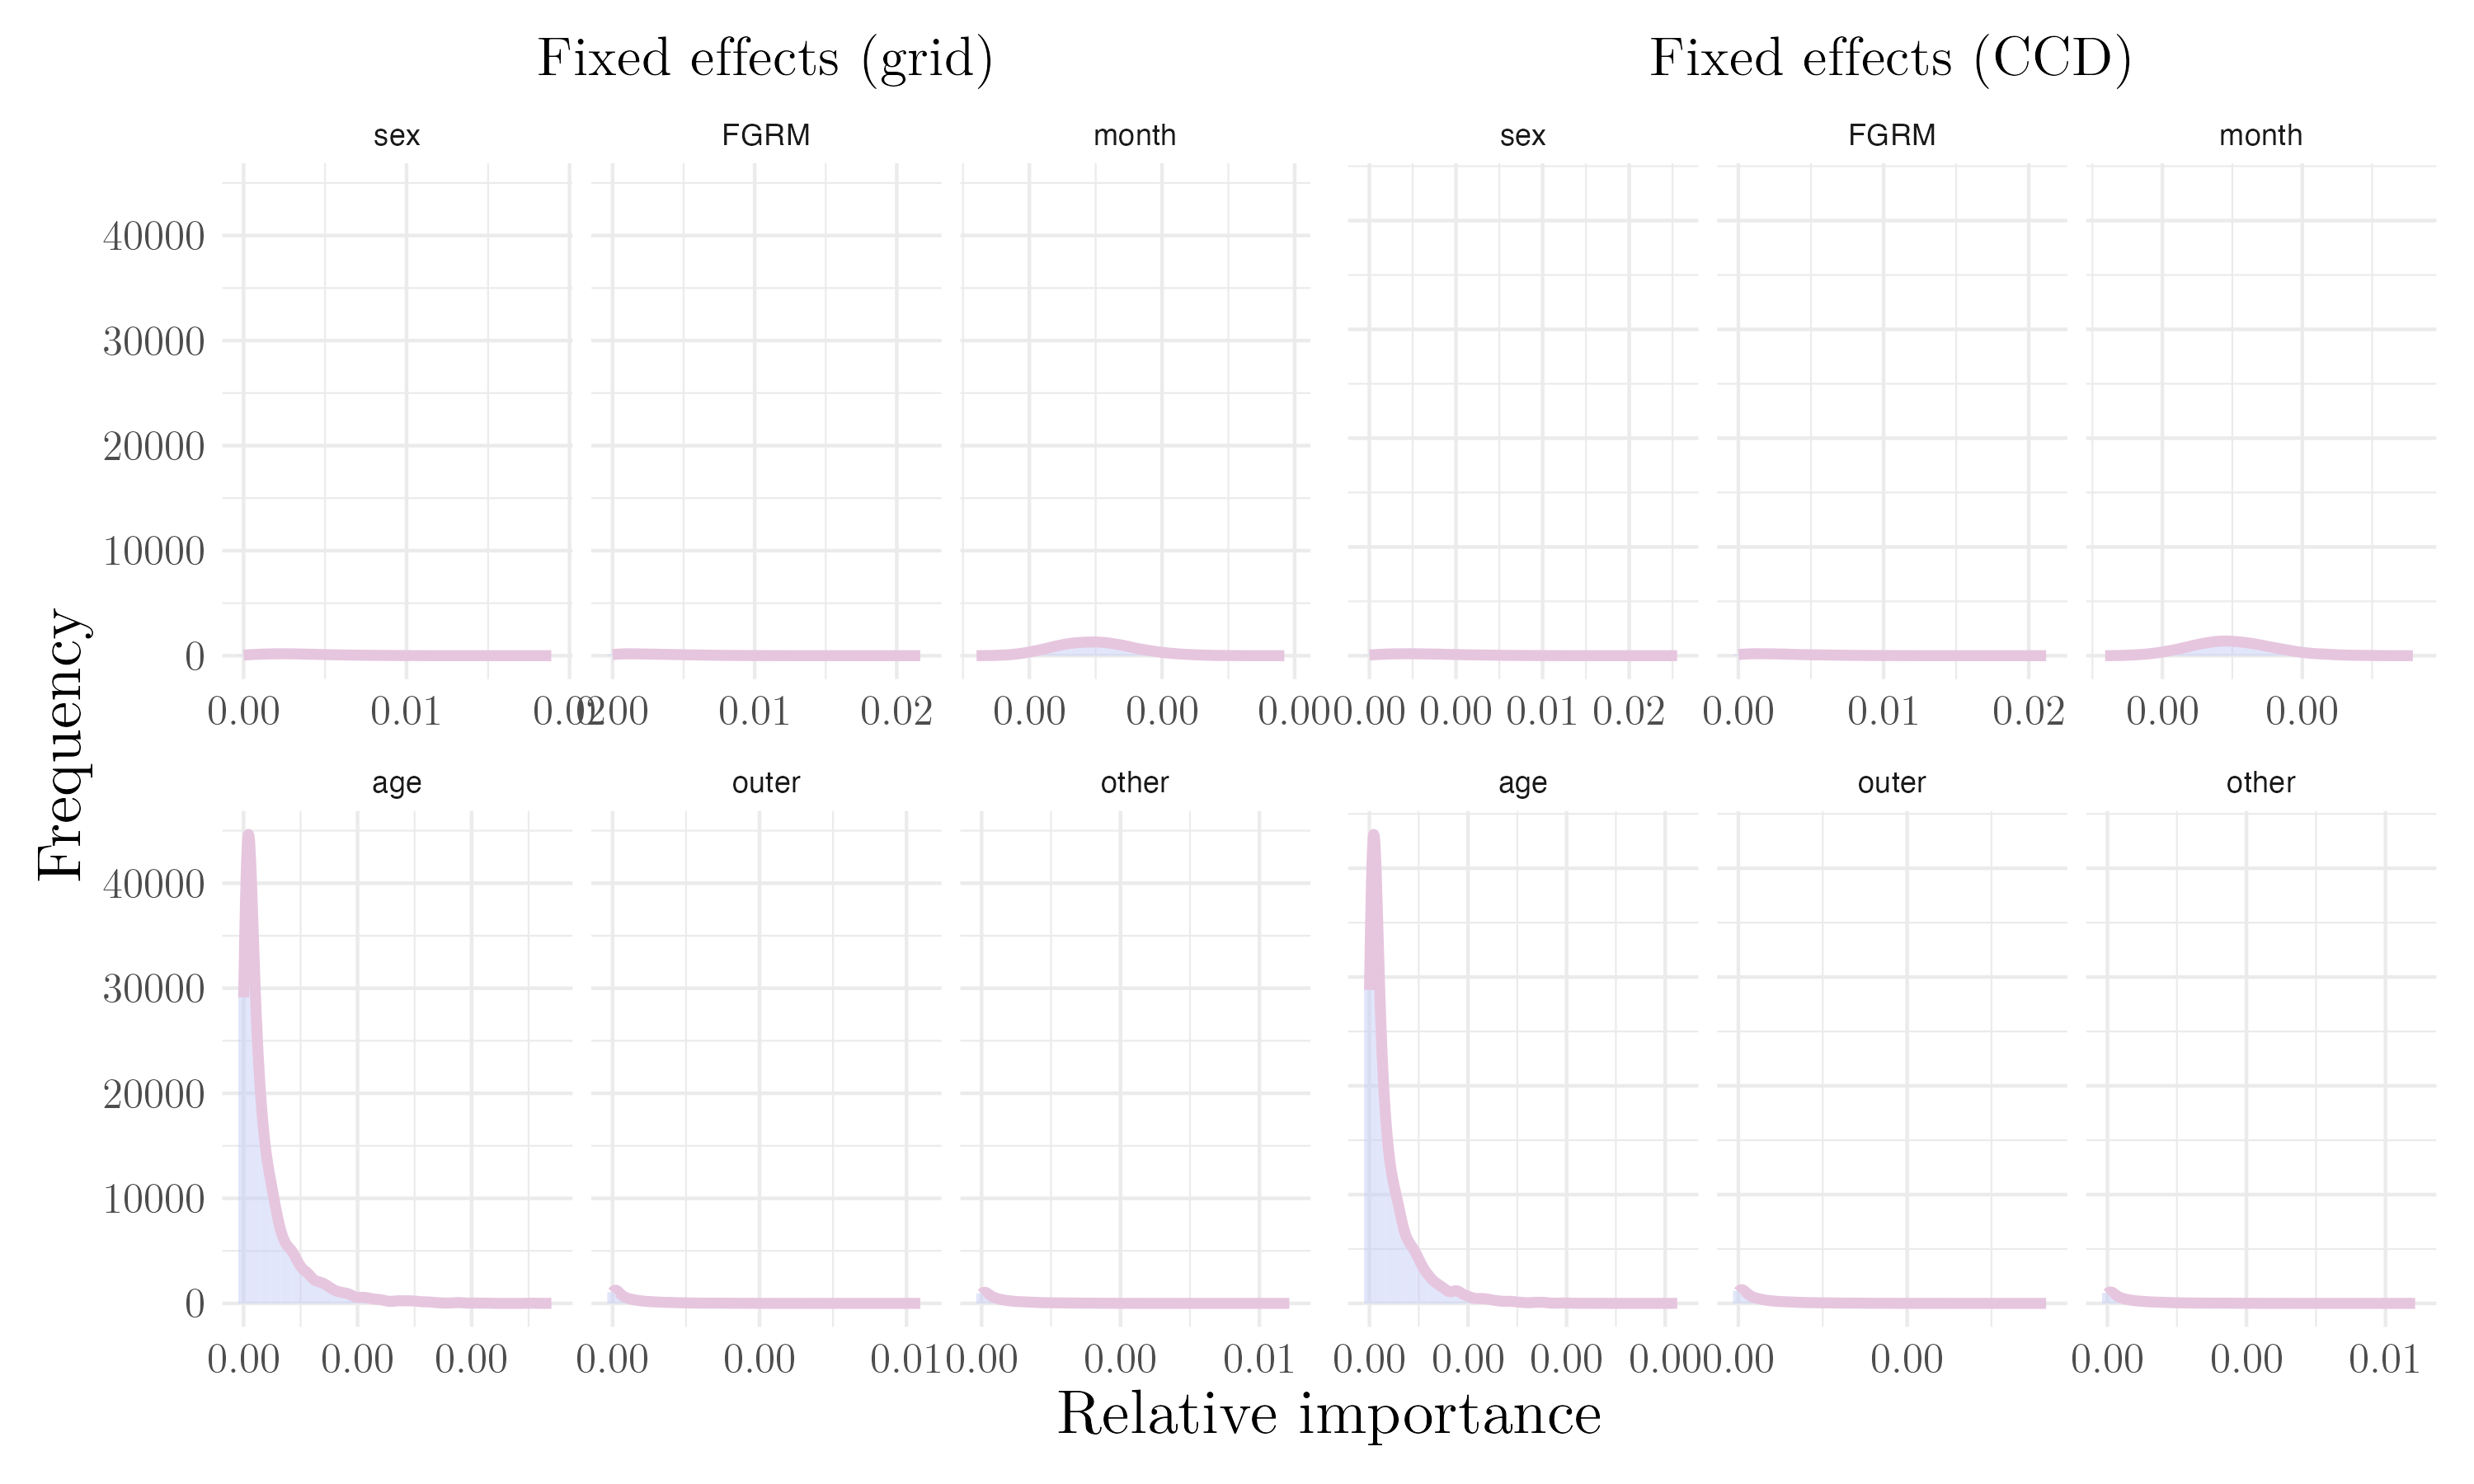
\includegraphics[width=1\linewidth]{Figures/House sparrow study/Tarsus_fixed.png}
  \caption[Posterior relative importance distributions of fixed effects in tarsus length model for house sparrow study]{Posterior relative importance distributions of fixed effects in tarsus length model for house sparrow study}
  \label{fig:tarsus_fixed_sparrows}
\end{figure}

\begin{figure}[H]%\ContinuedFloat
  \centering
  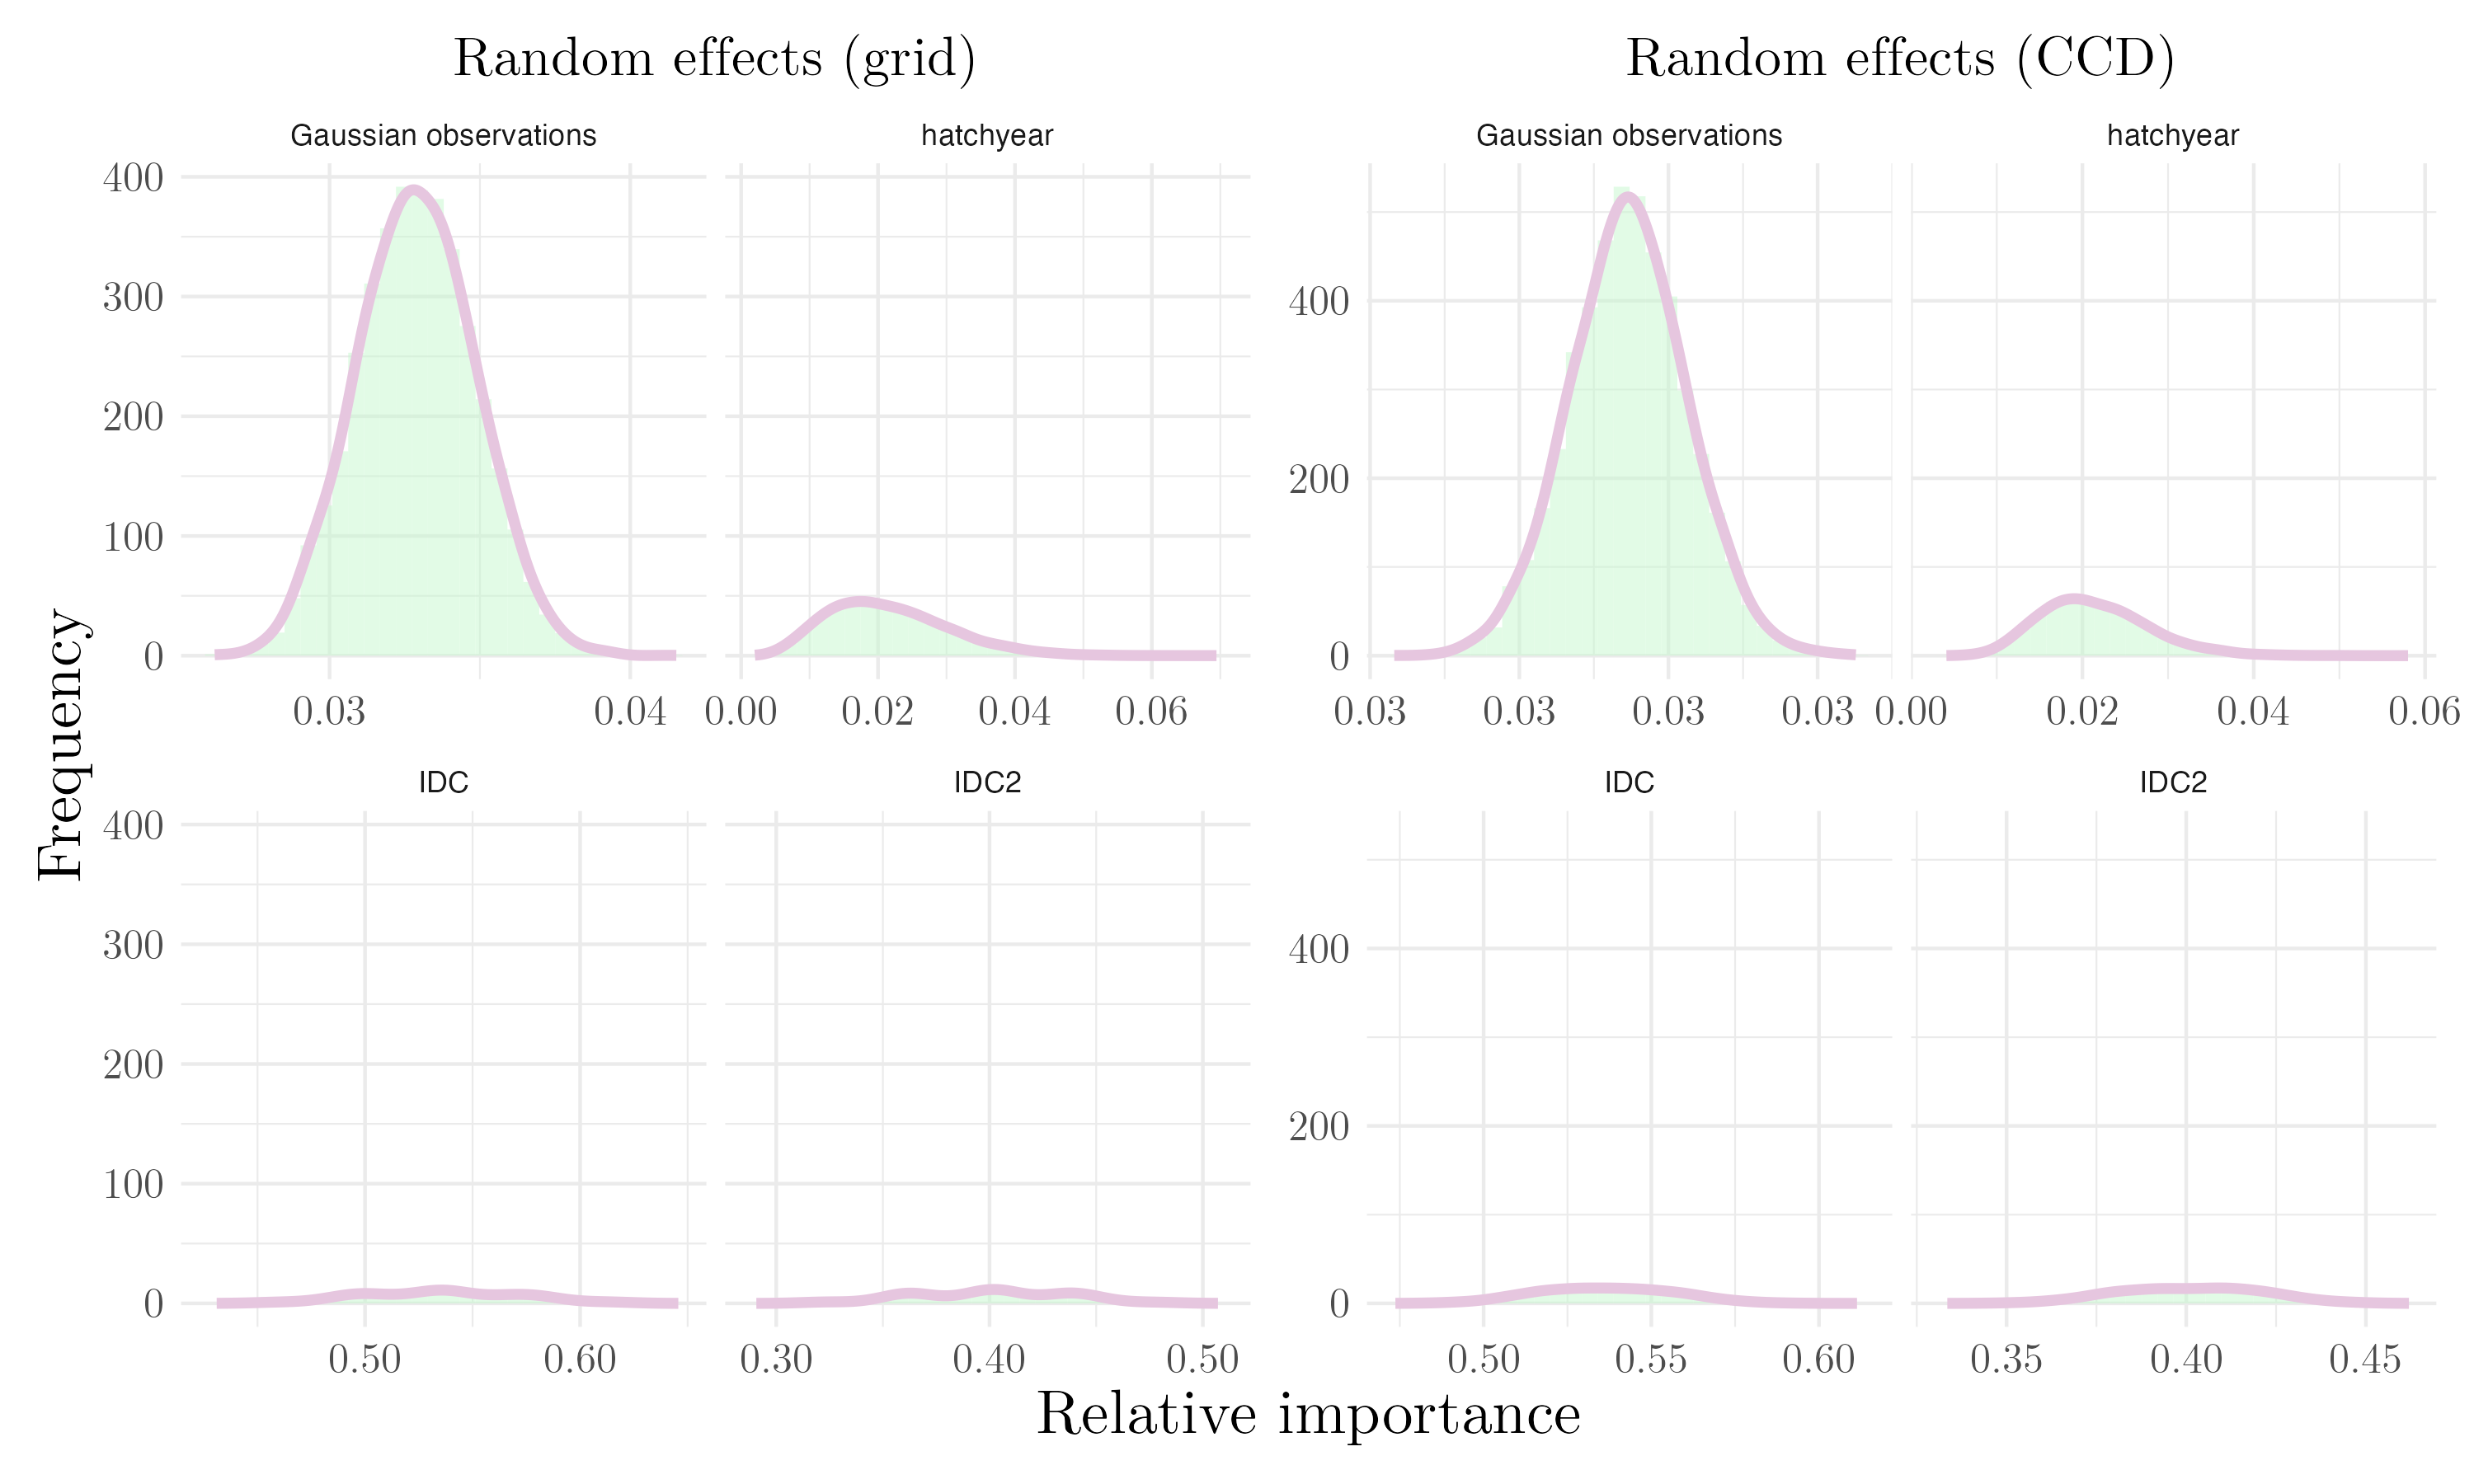
\includegraphics[width=1\linewidth]{Figures/House sparrow study/Tarsus_random.png}
  \caption[Posterior relative importance distributions of random effects in tarsus length model for house sparrow study]{Posterior relative importance distributions of random effects in tarsus length model for house sparrow study}
  \label{fig:tarsus_random_sparrows}
\end{figure}

\begin{figure}[H]%\ContinuedFloat
  \centering
  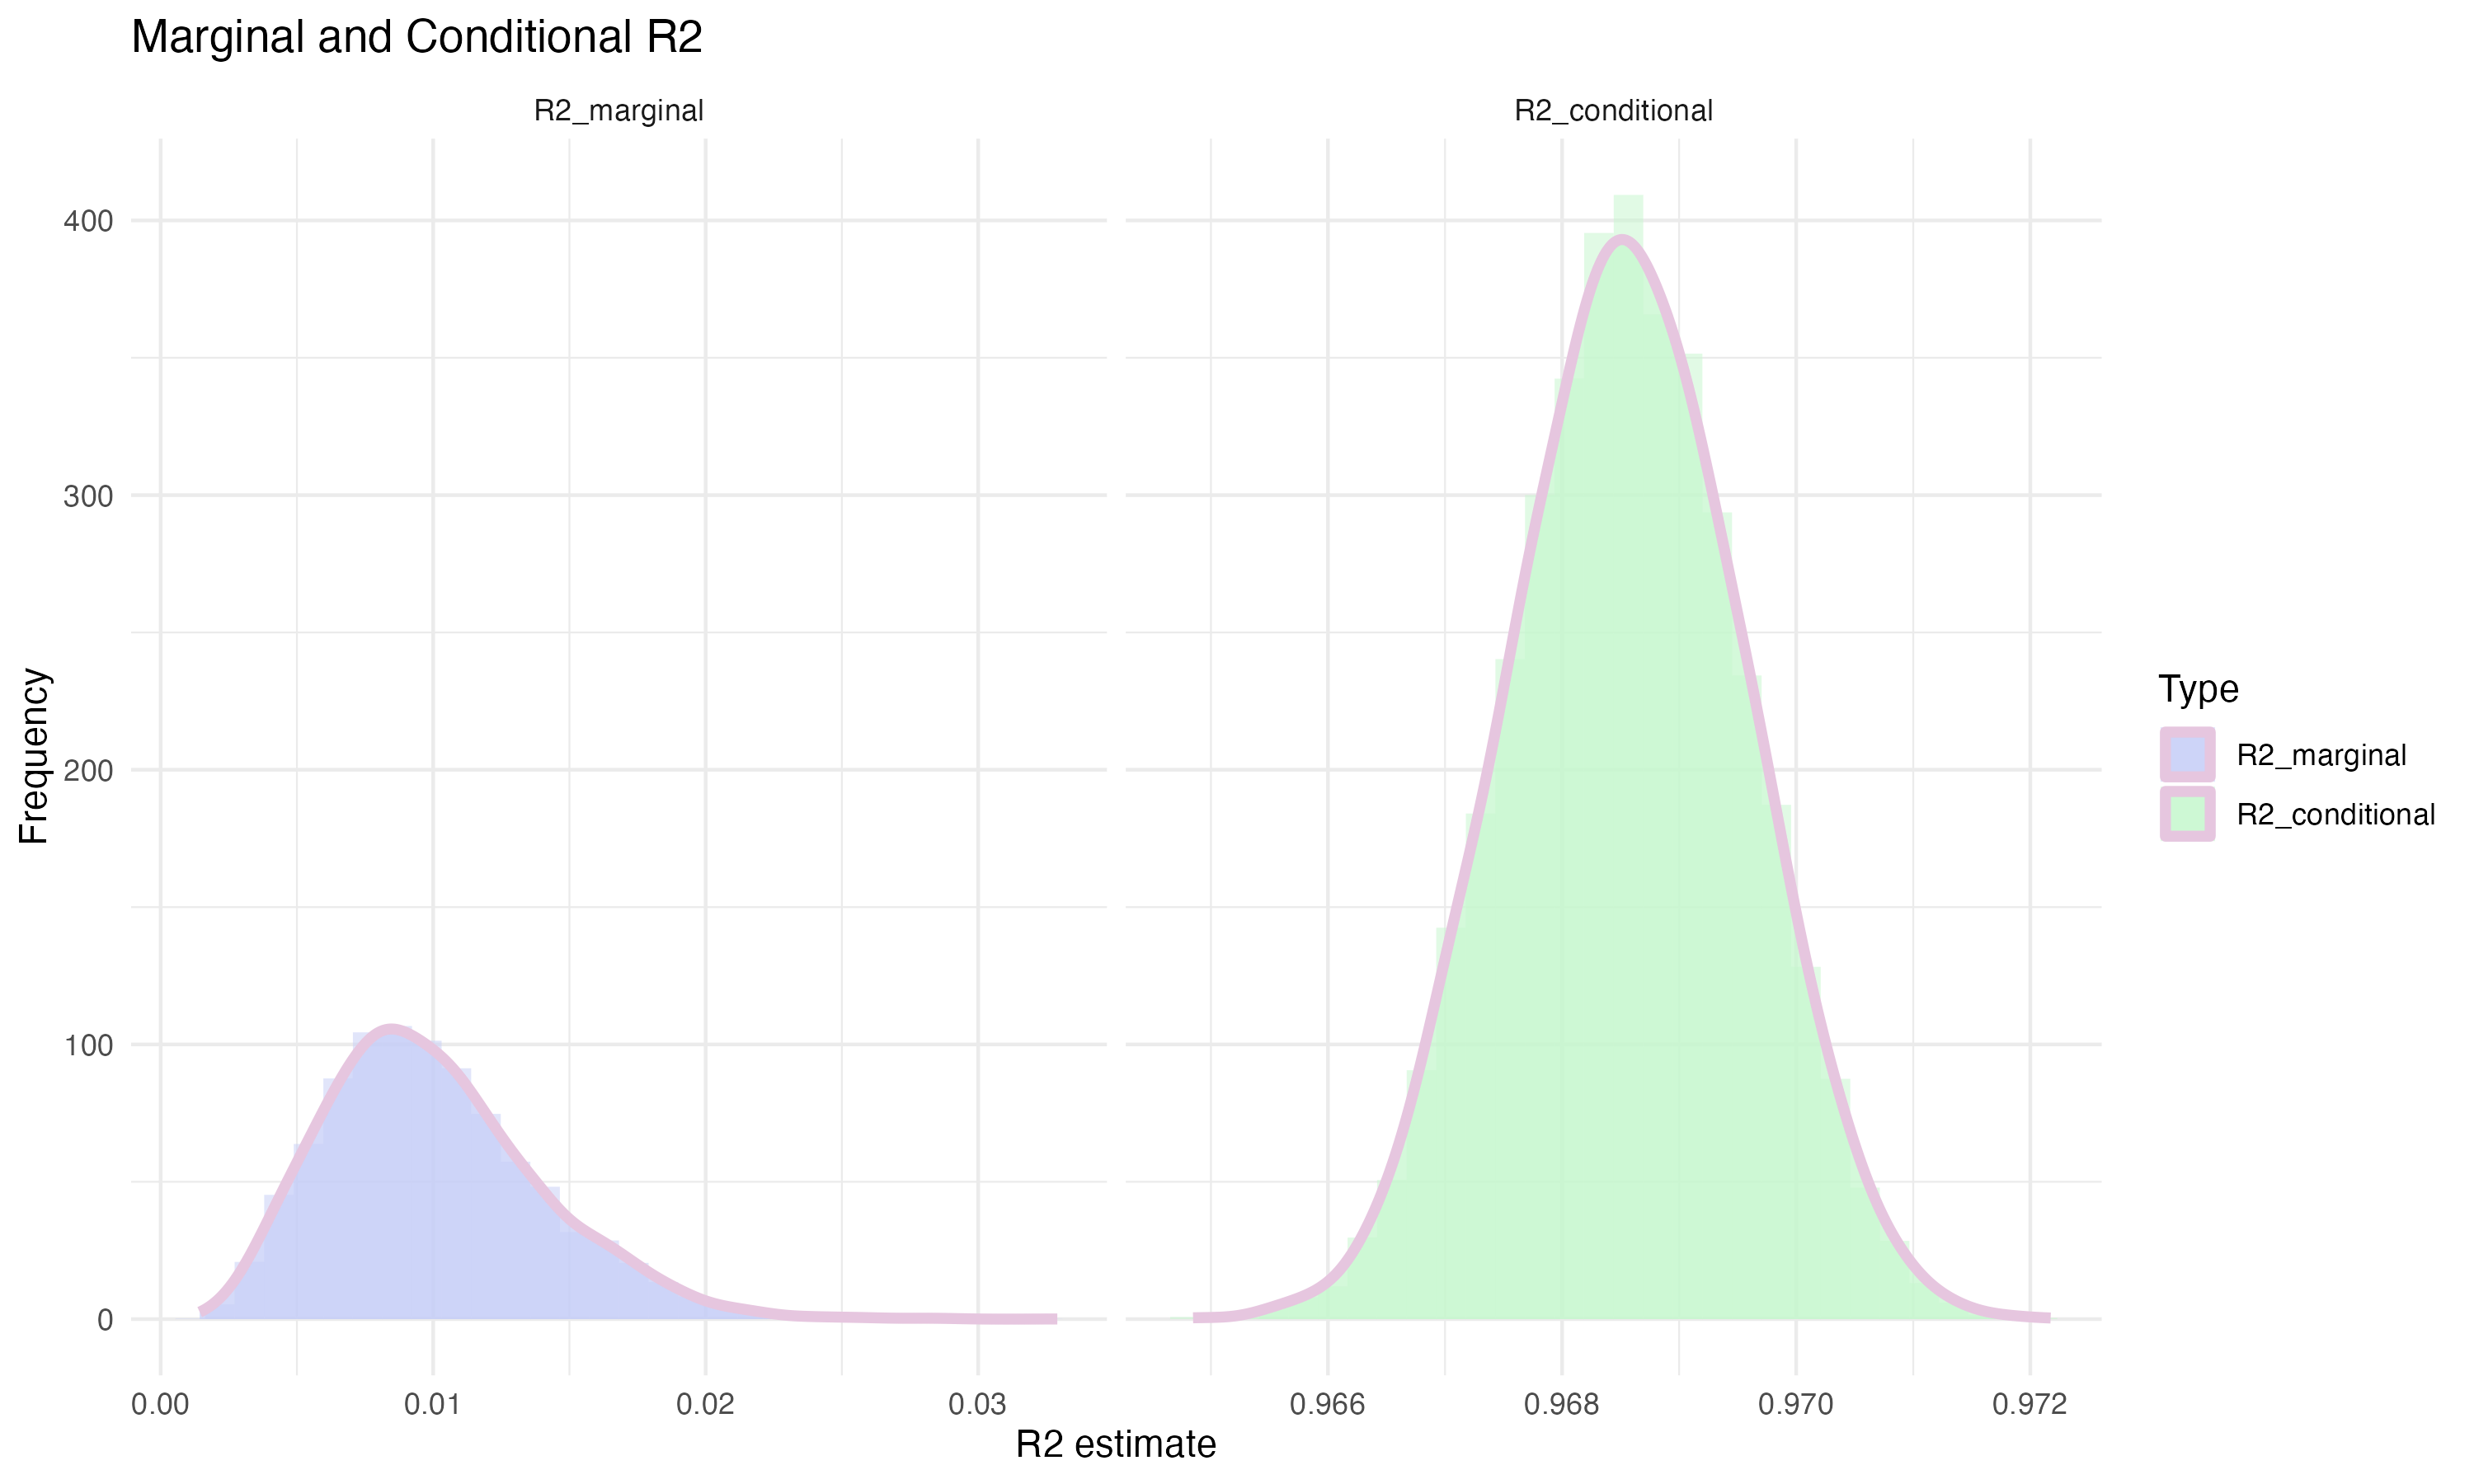
\includegraphics[width=1\linewidth]{Figures/House sparrow study/Tarsus_r2.png}
  \caption[Posterior distributions of $R^2$ values in tarsus length model for house sparrow study]{Posterior distributions of $R^2$ values in tarsus length model for house sparrow study}
  \label{fig:tarsus_r2}
\end{figure}

\subsection*{Supplementary tables for the non-Gaussian simulation study}
We attach the summarizing tables for the Binomial and Poisson simulation studies here, as they were referred to throughout the thesis. Firstly, \Cref{table:summary_logit} contains summary statistics of the distribution obtained from the Binomial model, while \Cref{table:summary_poisson} contains the same for the Poisson model.

\begin{table}[!ht]
    \centering
    \begin{tabular}{@{}llcccccc@{}}
      \toprule
      \multicolumn{2}{c}{\textbf{Measure}} & $\mathbf{\rho=0}$ & $\mathbf{\rho=0.1}$ & $\mathbf{\rho=-0.1}$ & $\mathbf{\rho=0.4}$ & $\mathbf{\rho=-0.4}$ \\ \midrule
      \multirow{3}{*}{\shortstack{Relative Importance of \\ Random effect}} & Average & 0.0947 & 0.0850 & 0.1079 & 0.0667 & 0.1694 \\
                                         & 2.5\%   & 0.0697 & 0.0609 & 0.0771 & 0.0488 & 0.1246 \\
                                         & 97.5\%  & 0.1223 & 0.1128 & 0.1420 & 0.0889 & 0.2153 \\ \midrule
      \multirow{3}{*}{\shortstack{Relative Importance of \\ Fixed effect X1}} & Average & 0.0978 & 0.1175 & 0.0774 & 0.1724 & 0.0200 \\
                                           & 2.5\%   & 0.0817 & 0.1025 & 0.0637 & 0.1580 & 0.0162 \\
                                           & 97.5\%  & 0.1134 & 0.1350 & 0.0917 & 0.1885 & 0.0245 \\ \midrule
      \multirow{3}{*}{\shortstack{Relative Importance of \\ Fixed effect X2}} & Average & 0.1951 & 0.2100 & 0.1763 & 0.2392 & 0.0769 \\
                                           & 2.5\%   & 0.1735 & 0.1903 & 0.1566 & 0.2206 & 0.0643 \\
                                           & 97.5\%  & 0.2155 & 0.2324 & 0.1956 & 0.2584 & 0.0911 \\ \midrule
      \multirow{3}{*}{\shortstack{Relative Importance of \\ Fixed effect X3}} & Average & 0.2922 & 0.2984 & 0.2795 & 0.2984 & 0.1666 \\
                                           & 2.5\%   & 0.2675 & 0.2742 & 0.2539 & 0.2770 & 0.1466 \\
                                           & 97.5\%  & 0.3187 & 0.3224 & 0.3047 & 0.3201 & 0.1909 \\ \midrule
      \multirow{3}{*}{$R^2_m$}            & Average & 0.5851 & 0.6258 & 0.5331 & 0.7100 & 0.2634 \\
                                           & 2.5\%   & 0.5549 & 0.5965 & 0.5023 & 0.6847 & 0.2357 \\
                                           & 97.5\%  & 0.6146 & 0.6552 & 0.5632 & 0.7360 & 0.2960 \\ \midrule
      \multirow{3}{*}{$R^2_c$}            & Average & 0.6799 & 0.7108 & 0.6411 & 0.7767 & 0.4328 \\
                                           & 2.5\%   & 0.6529 & 0.6865 & 0.6118 & 0.7555 & 0.3934 \\
                                           & 97.5\%  & 0.7046 & 0.7352 & 0.6677 & 0.7967 & 0.4729 \\ \bottomrule
    \end{tabular}
    % \begin{tabular}{@{}llcccccc@{}}
    %   \toprule
    %   \multicolumn{2}{c}{\textbf{Measure}} & $\mathbf{\rho=0}$ & $\mathbf{\rho=0.1}$ & $\mathbf{\rho=-0.1}$ & $\mathbf{\rho=0.4}$ & $\mathbf{\rho=-0.4}$ \\ \midrule
    %   \multirow{3}{*}{\shortstack{Relative Importance of \\ Random effect}} & Average & 0.0971 & 0.0861 & 0.1067 & 0.0663 & 0.1688 \\
    %                                      & 2.5\%   & 0.0732 & 0.0621 & 0.0796 & 0.0472 & 0.1266 \\
    %                                      & 97.5\%  & 0.1262 & 0.1148 & 0.1381 & 0.0885 & 0.2087 \\ \midrule
    %   \multirow{3}{*}{\shortstack{Relative Importance of \\ Fixed effect X1}} & Average & 0.0972 & 0.1170 & 0.0775 & 0.1728 & 0.0199 \\
    %                                        & 2.5\%   & 0.0824 & 0.1005 & 0.0643 & 0.1578 & 0.0168 \\
    %                                        & 97.5\%  & 0.1124 & 0.1326 & 0.0916 & 0.1873 & 0.0239 \\ \midrule
    %   \multirow{3}{*}{\shortstack{Relative Importance of \\ Fixed effect X2}} & Average & 0.1945 & 0.2103 & 0.1761 & 0.2390 & 0.0767 \\
    %                                        & 2.5\%   & 0.1731 & 0.1891 & 0.1541 & 0.2227 & 0.0632 \\
    %                                        & 97.5\%  & 0.2155 & 0.2323 & 0.1972 & 0.2584 & 0.0898 \\ \midrule
    %   \multirow{3}{*}{\shortstack{Relative Importance of \\ Fixed effect X3}} & Average & 0.2919 & 0.2983 & 0.2805 & 0.2991 & 0.1662 \\
    %                                        & 2.5\%   & 0.2653 & 0.2724 & 0.2571 & 0.2792 & 0.1456 \\
    %                                        & 97.5\%  & 0.3134 & 0.3229 & 0.3047 & 0.3183 & 0.1874 \\ \midrule
    %   \multirow{3}{*}{$R^2_m$}            & Average & 0.5836 & 0.6256 & 0.5342 & 0.7108 & 0.2628 \\
    %                                        & 2.5\%   & 0.5533 & 0.5951 & 0.5020 & 0.6850 & 0.2337 \\
    %                                        & 97.5\%  & 0.6119 & 0.6532 & 0.5648 & 0.7348 & 0.2918 \\ \midrule
    %   \multirow{3}{*}{$R^2_c$}            & Average & 0.6807 & 0.7117 & 0.6409 & 0.7772 & 0.4316 \\
    %                                        & 2.5\%   & 0.6512 & 0.6889 & 0.6132 & 0.7562 & 0.3944 \\
    %                                        & 97.5\%  & 0.7072 & 0.7354 & 0.6696 & 0.7971 & 0.4695 \\ \bottomrule
    % \end{tabular}    
    \caption[Summary statistics for binomial GLMM simulation study]{Summary of simulation study results for the quantiles of relative importance estimates of the Logit model across different correlation levels. For $\rho=0$ the expected values are given in \Cref{table:2}.}
    \label{table:summary_logit}
\end{table}

\begin{table}[H]
    \centering
    \begin{tabular}{@{}llcccccc@{}}
      \toprule
      \multicolumn{2}{c}{\textbf{Measure}} & $\mathbf{\rho=0}$ & $\mathbf{\rho=0.1}$ & $\mathbf{\rho=-0.1}$ & $\mathbf{\rho=0.4}$ & $\mathbf{\rho=-0.4}$ \\ \midrule
      \multirow{3}{*}{\shortstack{Relative Importance of \\ Random effect}} & Average & 0.0857 & 0.0781 & 0.0940 & 0.0627 & 0.1396 \\
                                         & 2.5\%   & 0.0642 & 0.0571 & 0.0679 & 0.0444 & 0.1002 \\
                                         & 97.5\%  & 0.1121 & 0.1023 & 0.1209 & 0.0809 & 0.1807 \\ \midrule
      \multirow{3}{*}{\shortstack{Relative Importance of \\ Fixed effect X1}} & Average & 0.0858 & 0.1045 & 0.0674 & 0.1579 & 0.0163 \\
                                           & 2.5\%   & 0.0751 & 0.0941 & 0.0582 & 0.1489 & 0.0138 \\
                                           & 97.5\%  & 0.0965 & 0.1149 & 0.0781 & 0.1671 & 0.0198 \\ \midrule
      \multirow{3}{*}{\shortstack{Relative Importance of \\ Fixed effect X2}} & Average & 0.1730 & 0.1874 & 0.1539 & 0.2192 & 0.0627 \\
                                           & 2.5\%   & 0.1594 & 0.1754 & 0.1395 & 0.2086 & 0.0525 \\
                                           & 97.5\%  & 0.1873 & 0.2006 & 0.1697 & 0.2301 & 0.0743 \\ \midrule
      \multirow{3}{*}{\shortstack{Relative Importance of \\ Fixed effect X3}} & Average & 0.2588 & 0.2677 & 0.2447 & 0.2740 & 0.1357 \\
                                           & 2.5\%   & 0.2423 & 0.2524 & 0.2277 & 0.2617 & 0.1197 \\
                                           & 97.5\%  & 0.2757 & 0.2831 & 0.2638 & 0.2851 & 0.1529 \\ \midrule
      \multirow{3}{*}{$R^2_m$}            & Average & 0.5176 & 0.5596 & 0.4660 & 0.6510 & 0.2147 \\
                                           & 2.5\%   & 0.4978 & 0.5377 & 0.4463 & 0.6339 & 0.1936 \\
                                           & 97.5\%  & 0.5355 & 0.5783 & 0.4878 & 0.6679 & 0.2361 \\ \midrule
      \multirow{3}{*}{$R^2_c$}            & Average & 0.6033 & 0.6378 & 0.5600 & 0.7138 & 0.3543 \\
                                           & 2.5\%   & 0.5815 & 0.6197 & 0.5350 & 0.6962 & 0.3181 \\
                                           & 97.5\%  & 0.6245 & 0.6597 & 0.5848 & 0.7290 & 0.3900 \\ \bottomrule
    \end{tabular}
    % \begin{tabular}{@{}llcccccc@{}}
    %   \toprule
    %   \multicolumn{2}{c}{\textbf{Measure}} & $\mathbf{\rho=0}$ & $\mathbf{\rho=0.1}$ & $\mathbf{\rho=-0.1}$ & $\mathbf{\rho=0.4}$ & $\mathbf{\rho=-0.4}$ \\ \midrule
    %   \multirow{3}{*}{\shortstack{Relative Importance of \\ Random effect}} & Average & 0.1348 & 0.1159 & 0.1560 & 0.0868 & 0.3299 \\
    %                                      & 2.5\%   & 0.1018 & 0.0914 & 0.1212 & 0.0600 & 0.2713 \\
    %                                      & 97.5\%  & 0.1689 & 0.1464 & 0.1931 & 0.1072 & 0.3903 \\ \midrule
    %   \multirow{3}{*}{\shortstack{Relative Importance of \\ Fixed effect X1}} & Average & 0.1337 & 0.1552 & 0.1112 & 0.2058 & 0.0385 \\
    %                                        & 2.5\%   & 0.1251 & 0.1478 & 0.1042 & 0.0002 & 0.0347 \\
    %                                        & 97.5\%  & 0.1421 & 0.1625 & 0.1195 & 0.2191 & 0.0425 \\ \midrule
    %   \multirow{3}{*}{\shortstack{Relative Importance of \\ Fixed effect X2}} & Average & 0.2672 & 0.2778 & 0.2544 & 0.2853 & 0.1489 \\
    %                                        & 2.5\%   & 0.2545 & 0.2647 & 0.2407 & 0.0002 & 0.1342 \\
    %                                        & 97.5\%  & 0.2803 & 0.2881 & 0.2679 & 0.3029 & 0.1648 \\ \midrule
    %   \multirow{3}{*}{\shortstack{Relative Importance of \\ Fixed effect X3}} & Average & 0.4008 & 0.3957 & 0.4039 & 0.3565 & 0.3237 \\
    %                                        & 2.5\%   & 0.3851 & 0.3799 & 0.3838 & 0.0003 & 0.2939 \\
    %                                        & 97.5\%  & 0.4185 & 0.4095 & 0.4222 & 0.3784 & 0.3576 \\ \midrule
    %   \multirow{3}{*}{$R^2_m$}            & Average & 0.8017 & 0.8286 & 0.7695 & 0.8476 & 0.5111 \\
    %                                        & 2.5\%   & 0.7722 & 0.7981 & 0.7363 & 0.0007 & 0.4639 \\
    %                                        & 97.5\%  & 0.8304 & 0.8530 & 0.8029 & 0.8960 & 0.5582 \\ \midrule
    %   \multirow{3}{*}{$R^2_c$}            & Average & 0.9365 & 0.9445 & 0.9255 & 0.9344 & 0.8410 \\
    %                                        & 2.5\%   & 0.9258 & 0.9354 & 0.9136 & 0.2112 & 0.8149 \\
    %                                        & 97.5\%  & 0.9467 & 0.9532 & 0.9358 & 0.9660 & 0.8658 \\ \bottomrule
    %   \end{tabular}
    \caption[Summary statistics for Poisson GLMM simulation study]{Summary of simulation study results for the quantiles of relative importance estimates the Poisson model across different correlation levels. For $\rho=0$ the expected values are given in \Cref{table:2}.}
    \label{table:summary_poisson}
  \end{table}
